\documentclass[12pt]{report}
\usepackage[dvips]{graphicx}
\graphicspath{{./}}
\usepackage[utf8]{inputenc}
\usepackage[russian]{babel}
\usepackage{listings}
\usepackage{longtable}
\usepackage{multirow} 

\usepackage{enumitem}
\usepackage{pdfpages}
\documentclass[14pt, a4paper]{article}
\usepackage[14pt]{extsizes}
\usepackage[utf8]{inputenc}
\usepackage[T2A]{fontenc}
\usepackage[english, russian]{babel}
\usepackage{setspace,amsmath}
\usepackage{amsfonts}
\usepackage{amssymb}
\usepackage{makeidx}
\usepackage{longtable}
\usepackage[left=30mm, top=15mm, right=10mm, bottom=15mm, nohead, footskip=10mm]{geometry}
\usepackage{lscape}

\addto\captionsrussian{\def\refname{Список используемой литературы}}

\usepackage{listings}

\usepackage{float}

\usepackage{wrapfig}
\usepackage{graphicx}
\usepackage{caption}
\graphicspath{{images/}}
\DeclareGraphicsExtensions{.pdf,.png,.jpg}

\setlength{\parindent}{4ex}
\usepackage{indentfirst}

\usepackage{hyperref}
\usepackage{cleveref}

\usepackage{titlesec, blindtext, xcolor, tcolorbox} 
\definecolor{blue}{rgb}{0,0,1} 
\newcommand{\hsp}{\hspace{20pt}} 

\titleformat{\chapter}{\LARGE\bfseries}{\thechapter}{20pt}{\huge\bfseries}
\titleformat{\section}{\Large\bfseries}{\thesection}{20pt}{\large\bfseries}

\lstset{upquote=true}

\lstdefinestyle{mystyle}{
    numberstyle=\numberstyle,
    basicstyle=\footnotesize\ttfamily,
    breakatwhitespace=false,
    breaklines=true,
    captionpos=b,
    keepspaces=true,
    numbers=none,
    numbersep=10pt,
    showspaces=false,
    showstringspaces=false,
    showtabs=false,
    frame=single,
    captionpos=t,
    language=prolog,
}
\lstset{style=mystyle}
\usepackage{pgfplots}
\usepackage{filecontents}
\usetikzlibrary{datavisualization}
\usetikzlibrary{datavisualization.formats.functions}

\begin{filecontents}{R1.dat}
250 1.40547e+07
300 1.45677e+07
350 1.48406e+07
400 1.5759e+07
450 1.60429e+07
500 1.6994e+07
550 1.76546e+07
600 1.77744e+07
650 1.82183e+07
\end{filecontents}

\begin{filecontents}{R2.dat}
1 1.5207e+07
2 1.52689e+07
3 1.56516e+07
4 1.59065e+07
5 1.6065e+07
\end{filecontents}

\begin{document}
\begin{titlepage}
	\newgeometry{left=3cm, right=1cm, top=2cm, bottom=2cm}
	\fontsize{12pt}{12pt}\selectfont
	\noindent \begin{minipage}{0.15\textwidth}
		
\includegraphics[width=\linewidth]{logo.jpg}
	\end{minipage}
	\noindent\begin{minipage}{0.8\textwidth}\centering
		\textbf{Министерство науки и высшего образования Российской Федерации}\\
		\textbf{Федеральное государственное бюджетное образовательное учреждение высшего образования}\\
		\textbf{«Московский государственный технический университет имени Н.Э.~Баумана}\\
		\textbf{(национальный исследовательский университет)»}\\
		\textbf{(МГТУ им. Н.Э.~Баумана)}
	\end{minipage}
	
	\noindent\rule{17cm}{3pt}
	\newline\newline
	\noindent ФАКУЛЬТЕТ $\underline{\text{«Информатика и системы управления»}}$ \newline\newline
	\noindent КАФЕДРА $\underline{\text{«Программное обеспечение ЭВМ и информационные технологии»}}$\newline\newline\newline\newline\newline\newline\newline
	
	
	\begin{center}
	\Large\textbf{Отчет}
	
	\large\textbf{\newlineК РЕАЛИЗАЦИИ РЕШЕНИЯ НА PROLOG \newline пасьянса «Свободная ячейка»}
    

	

	\end{center}
    
    ~ \\
    ~ \\
    ~ \\ 
    ~ \\
    ~ \\
    ~ \\
    
    $\text{Студент  } \underset{\text{(Группа)}}{\underline{\hspace{0.13\textwidth}}}$
    \hspace{0.3\textwidth}
    $\underset{\text{(Подпись, дата)}}{\underline{\hspace{0.13\textwidth}}}$
    \hspace{0.08\textwidth}
    \underset{\rm \text{(И.О. Фамилия)}}{\rm \text{Коваленко И.А.}}
    
    ~ \\
    ~ \\
    
    $\text{Студент  } \underset{\text{(Группа)}}{\underline{\hspace{0.13\textwidth}}}$
    \hspace{0.3\textwidth}
    $\underset{\text{(Подпись, дата)}}{\underline{\hspace{0.13\textwidth}}}$
    \hspace{0.08\textwidth}
    \underset{\rm \text{(И.О. Фамилия)}}{\rm \text{Кобаренков И.В.}}
    
    ~ \\
    ~ \\
    
    $\text{Руководитель проекта     }$
    \hspace{0.165\textwidth}
    $\underset{\text{(Подпись, дата)}}{\underline{\hspace{0.13\textwidth}}}$
    \hspace{0.08\textwidth}
    \underset{\rm \text{(И.О. Фамилия)}}{\rm \text{Строганов Ю.В.}}
	
	\begin{center}
	\vfill
	\the\year
	~г.
	\end{center}
	
 \restoregeometry
\end{titlepage}

\setcounter{page}{2}
\newpage
\tableofcontents

\newpage
\chapter*{Правила игры «Свободная ячейка»}

\addcontentsline{toc}{chapter}{Правила игры «Свободная ячейка»}
Используется колода карт из n цветов и m карт. Раскладывается вся колода в количество столбцов n * 2. Также есть n ячеек, именуемых «домом», и n «свободных» ячеек. В начале игры все они пусты. Разрешено перекладывать одну карту из колонки или свободной ячейки:

\begin{itemize}
	\item в любую другую колонку — на следующую по старшинству карту другого цвета;
	
	На рисунке 1 представлен пример данного шага.
        \begin{figure}[H]
            	\begin{center}
            		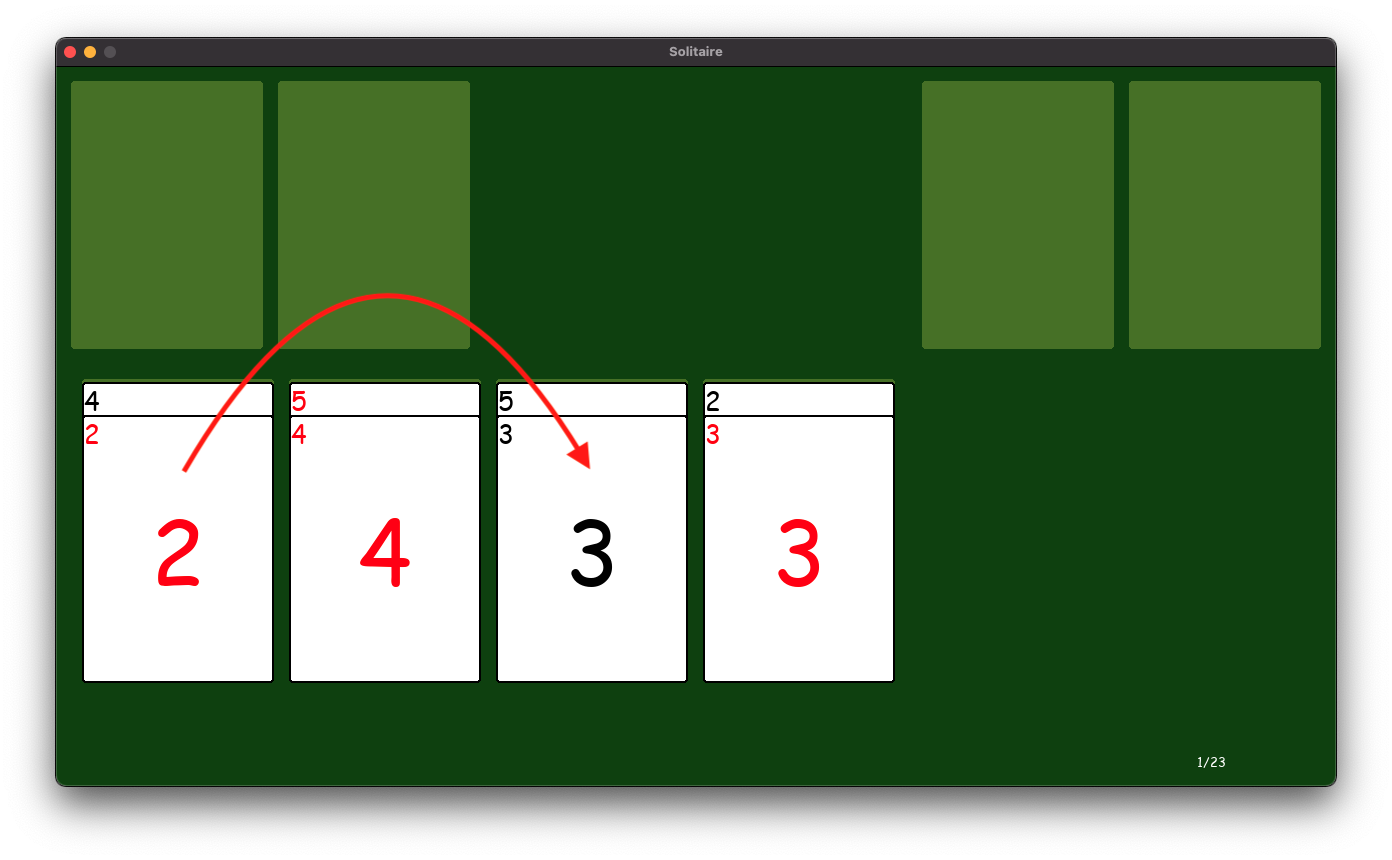
\includegraphics[scale=0.25]{prolog_1.png}
            		\caption{пример перемещения карты в любую другую колонку — на следующую по старшинству карту другого цвета}
            	\end{center}
        \end{figure}

	\item либо на свободную ячейку, если она пуста (таким образом, каждая из свободных ячеек может хранить только одну карту);
	
		На рисунке 2 представлен пример данного шага.
        \begin{figure}[H]
            	\begin{center}
            		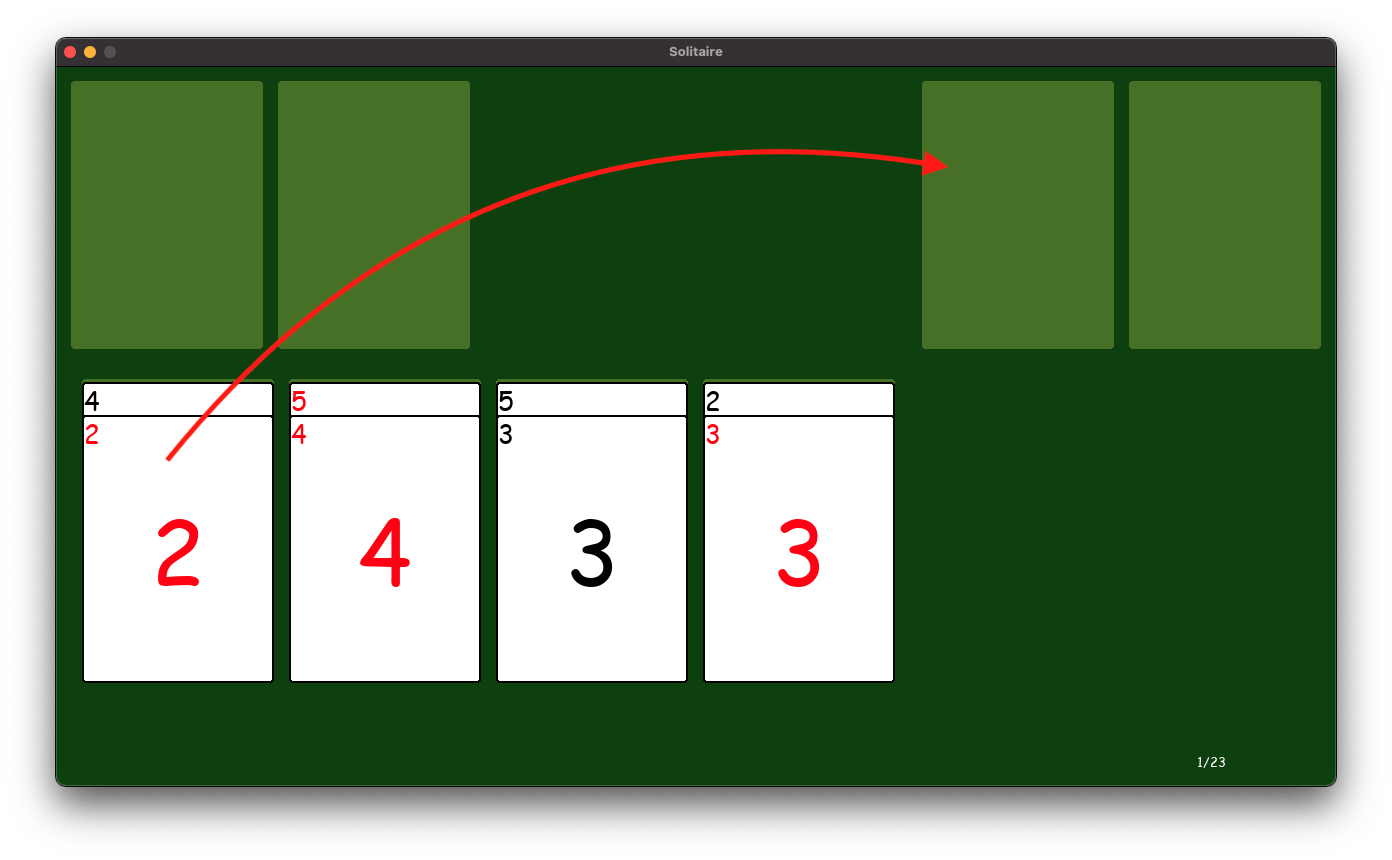
\includegraphics[scale=0.25]{prolog_2.png}
            		\caption{пример перемещения карты на свободную ячейку, если она пуста}
            	\end{center}
        \end{figure}

	\item либо в пустую колонку — без ограничений;
	
		На рисунке 3 представлен пример данного шага.
        \begin{figure}[H]
            	\begin{center}
            		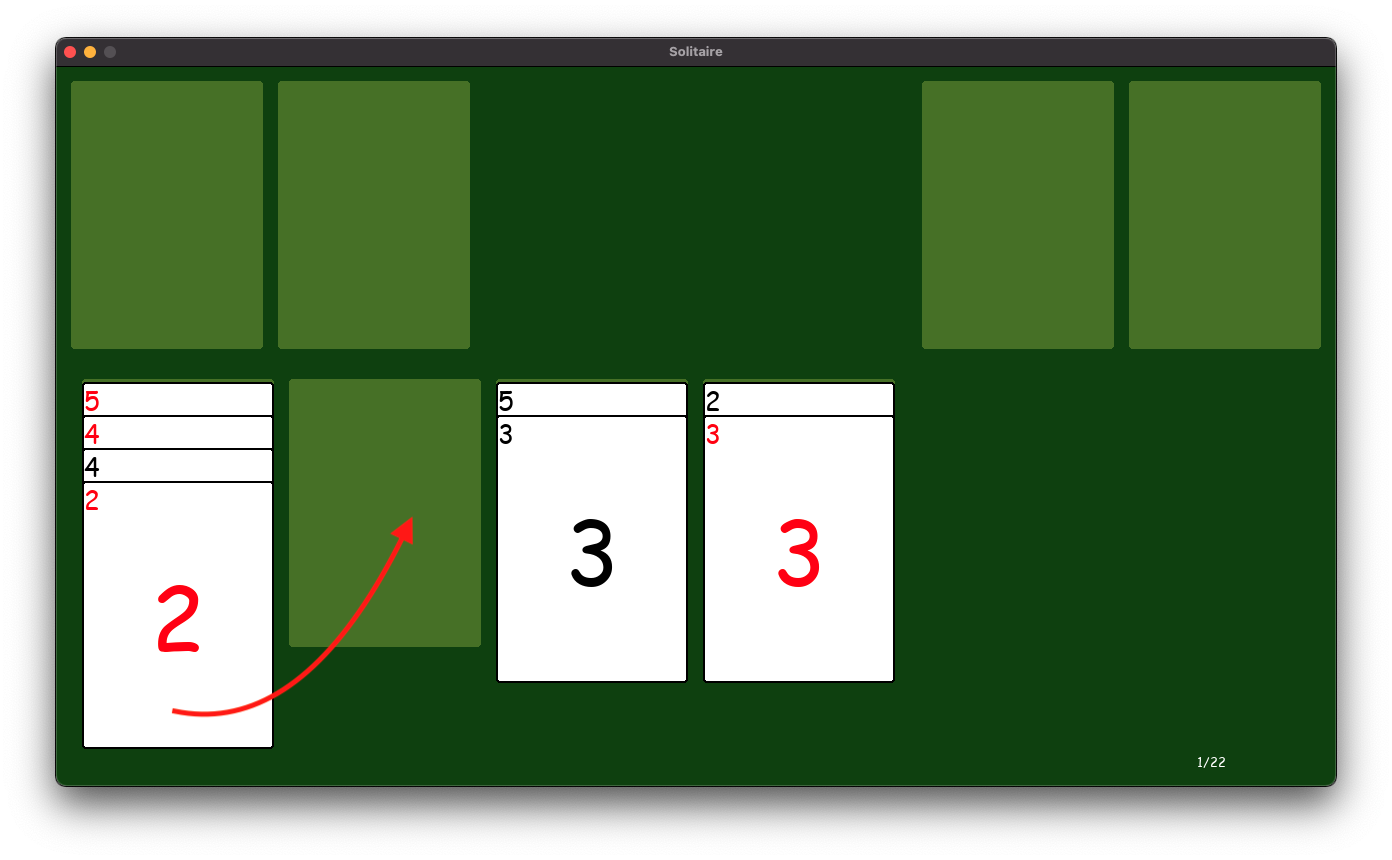
\includegraphics[scale=0.25]{prolog_6.png}
            		\caption{пример перемещения карты в пустую колонку}
            	\end{center}
        \end{figure}
	\item либо в «дом» — карты одной масти, начиная с самой старшей и дальше от младшей к старшей;
	
    	На рисунке 4 представлен пример данного шага.
        \begin{figure}[H]
            	\begin{center}
            		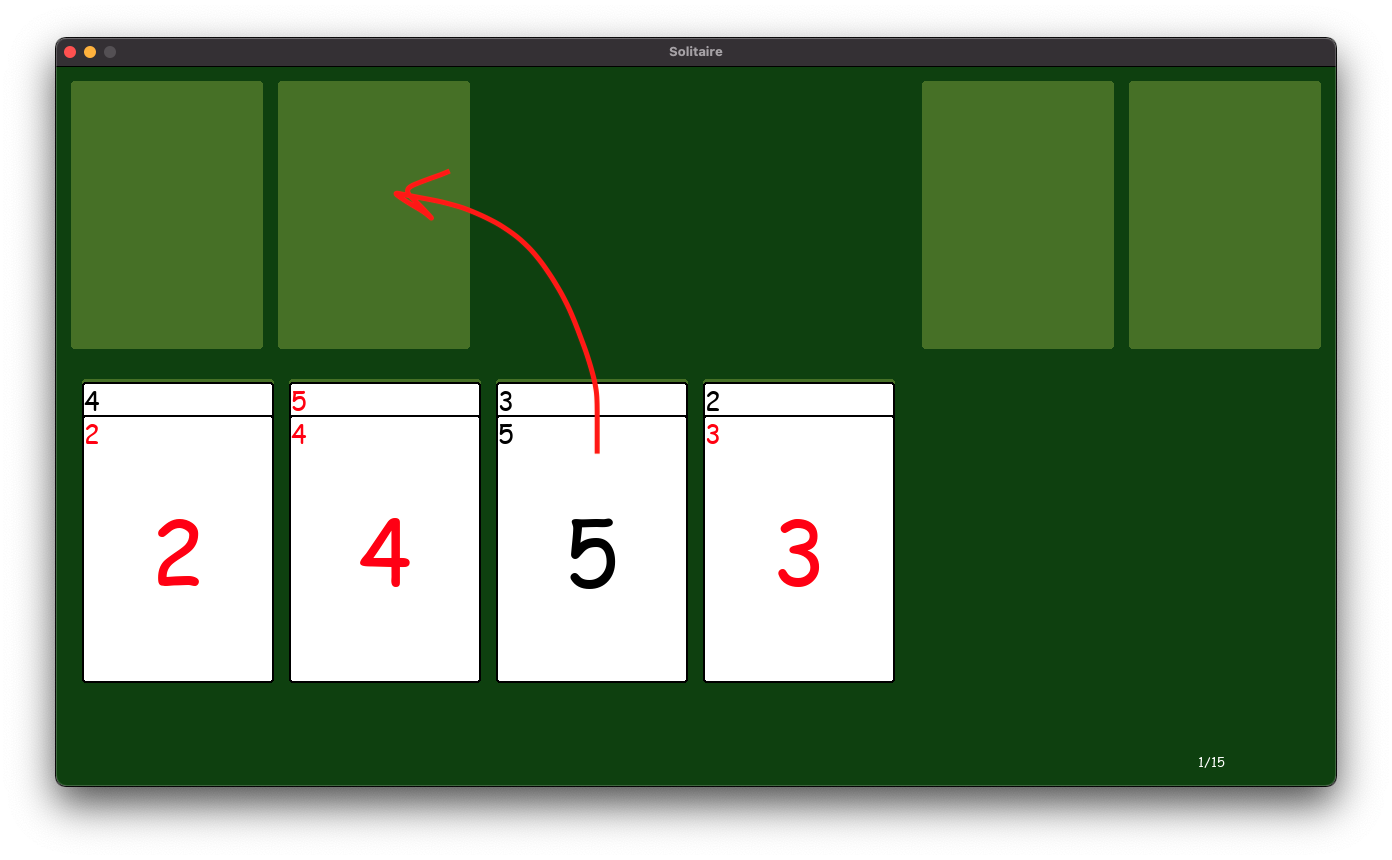
\includegraphics[scale=0.25]{prolog_5.png}
            		\caption{пример перемещения карты в «дом»}
            	\end{center}
        \end{figure}
	\item Если нужно перенести стопку карт, это можно сделать только по одной, используя пустые колонки и свободные ячейки.
\end{itemize}

Пасьянс сходится, если удаётся переместить всю колоду в «дом».

\newpage
\chapter*{Цель проекта}

\addcontentsline{toc}{chapter}{Цель проекта}

\parЦелью  проекта является разработка программного обеспечения для получения решения пасьянса  «Свободная ячейка» и визуализации найденного решения.

\parДля реализации поставленной задачи, необходимо выполнить следующие шаги:
\begin{itemize}
	\item провести анализ существующих решений;
	\item разработать программу поиска решения на языке Prolog;
	\item разработать GUI для визуализации найденного решения.
\end{itemize}
\chapter{Анализ существующих решений}
В результате поиска существующих решений для пасьянса «Свободная ячейка», было обнаружено, что над данной проблемой работает только один разработчик.[1]

На данной проблемой он работает уже более 14 лет, им было внесено более 11500 изменений в репозиторий проекта.

В результате проделанной работы им была создана программа и библиотека на языке C, позволяющая решать пасьянс «Свободная ячейка» и похожие на него другие разновидности пасьянса. 

\chapter{Выбор языка программирования}
Логический поиск решения было необходимо реализовать на языке логического программирования SWI-Prolog.

Для создания GUI было решено использовать Python, поскольку существует модуль для связи кода Python с кодом SWI-Prolog - Pyswip[4].
Для создания самого GUI использовался стандартный модуль Python - pygame[3].
Передача данных между Prolog'ом и Python'ом происходит в формате JSON.
\chapter{Основная проблема}
В ходе разработки было обнаружено, что часто программа зацикливается.

Было определено, что проблема в бесконечных повторении одних и тех же равноценных ходов. 

Например, если одна карта будет постоянно перемещаться между двумя конкретными столбцами. 

Для решения этой проблемы в программу было добавлено хранение набора состояний. После каждого нового сделанного хода, состояние полей игры сохраняется и поиск решения продолжается. Если же данное состояние уже добавлено в набор, ход не засчитывается и поиск продолжается дальше.

На рисунках 3.1-3.4 представлен пример ситуации зацикливания.
\begin{figure}[H]
    	\begin{center}
    		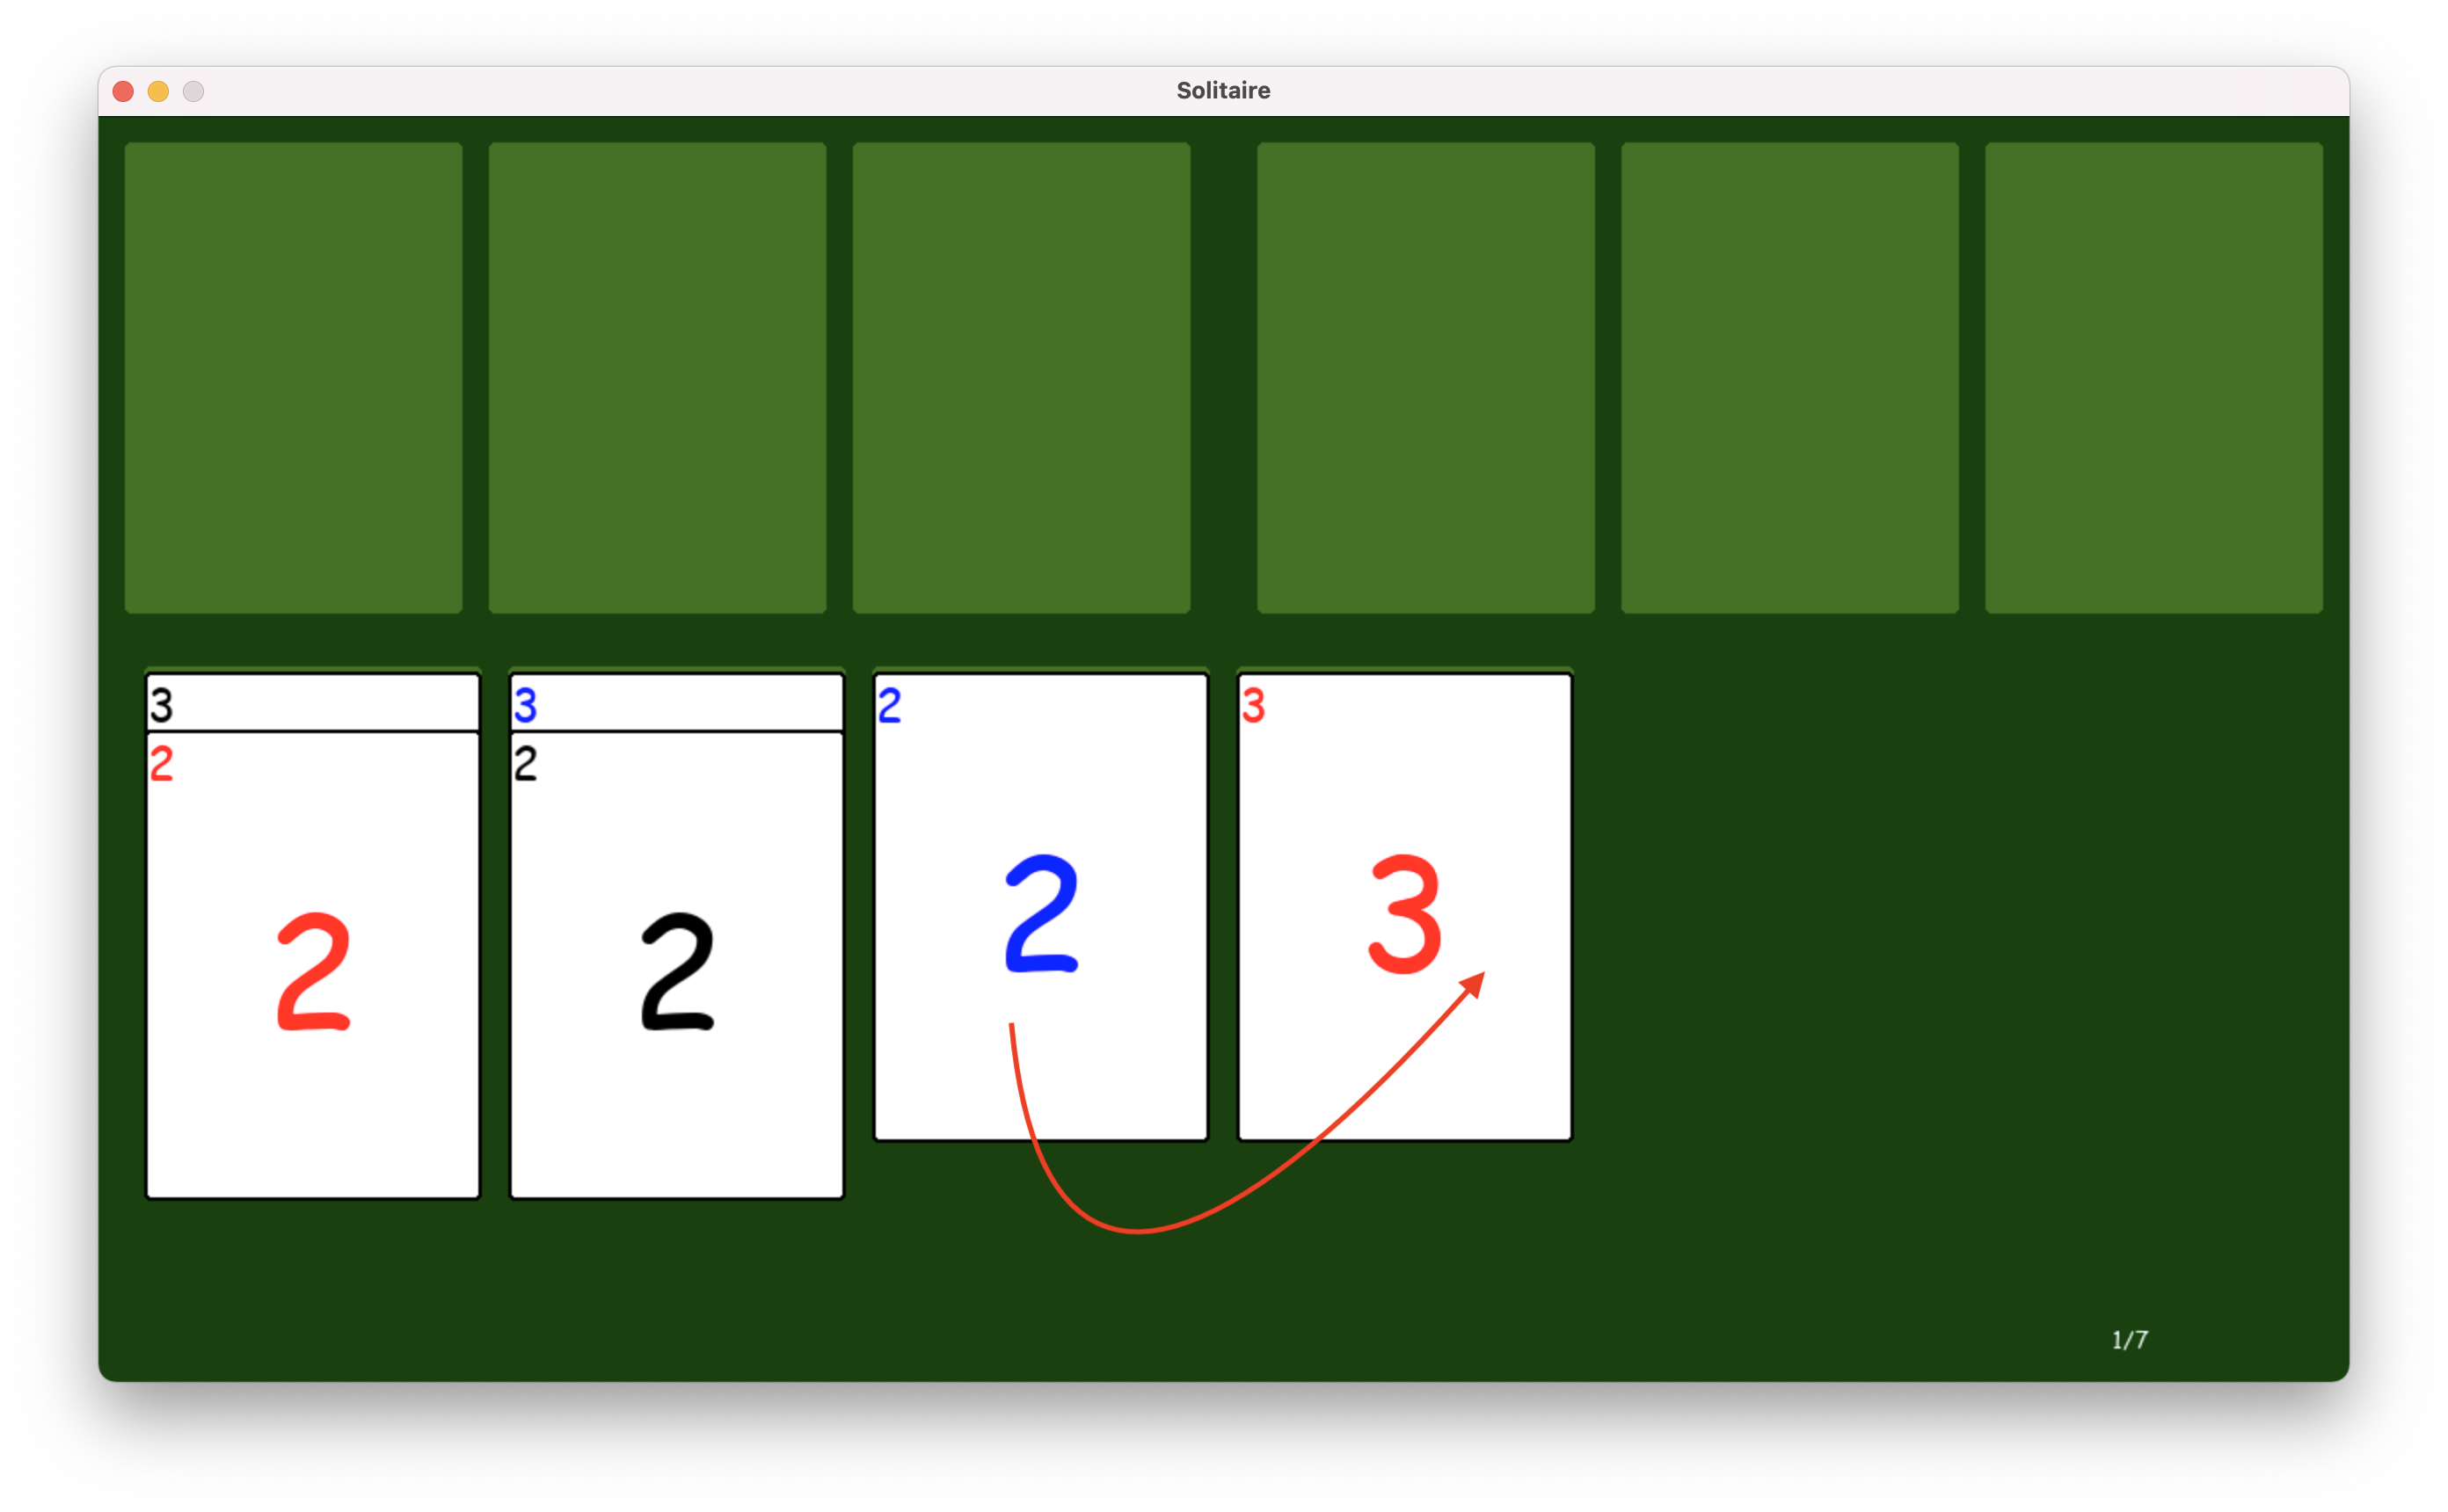
\includegraphics[scale=0.25]{problem_1.png}
    		\caption{перемещение синей двойки на красную тройку}
    	\end{center}
\end{figure}
\begin{figure}[H]
    	\begin{center}
    		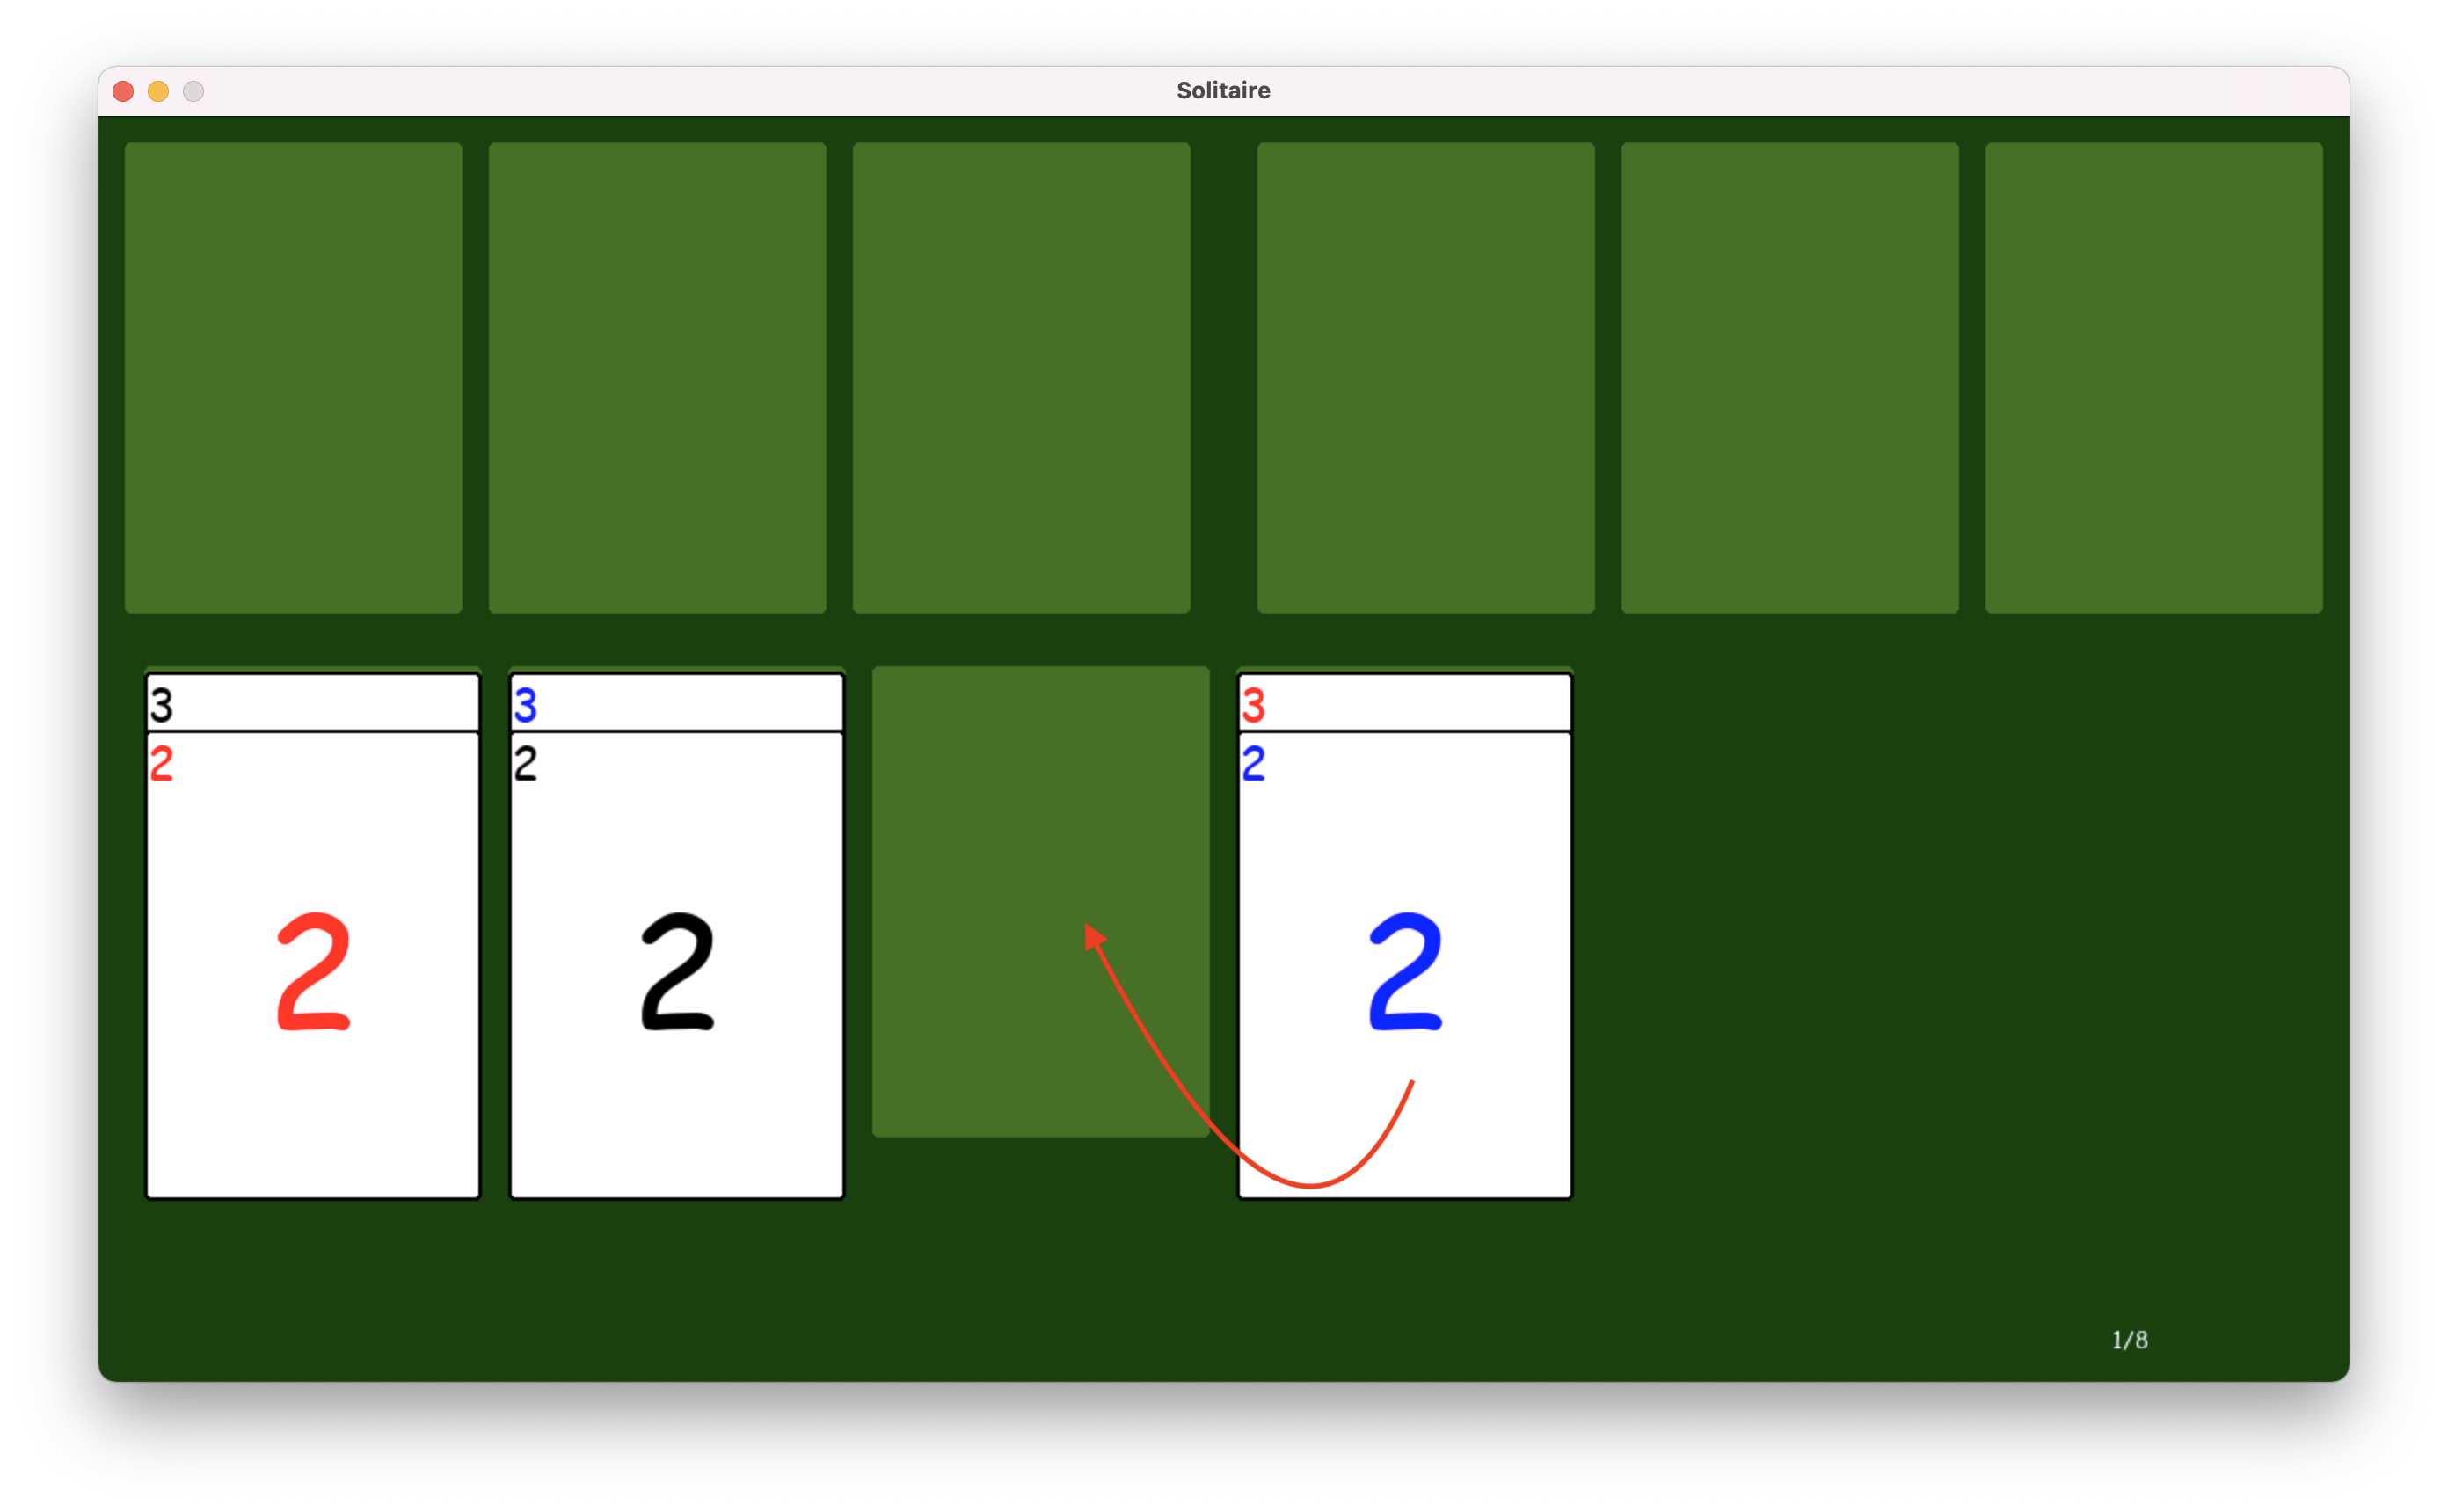
\includegraphics[scale=0.25]{problem_2.png}
    		\caption{перемещение синей двойки в пустой столбец}
    	\end{center}
\end{figure}
\begin{figure}[H]
    	\begin{center}
    		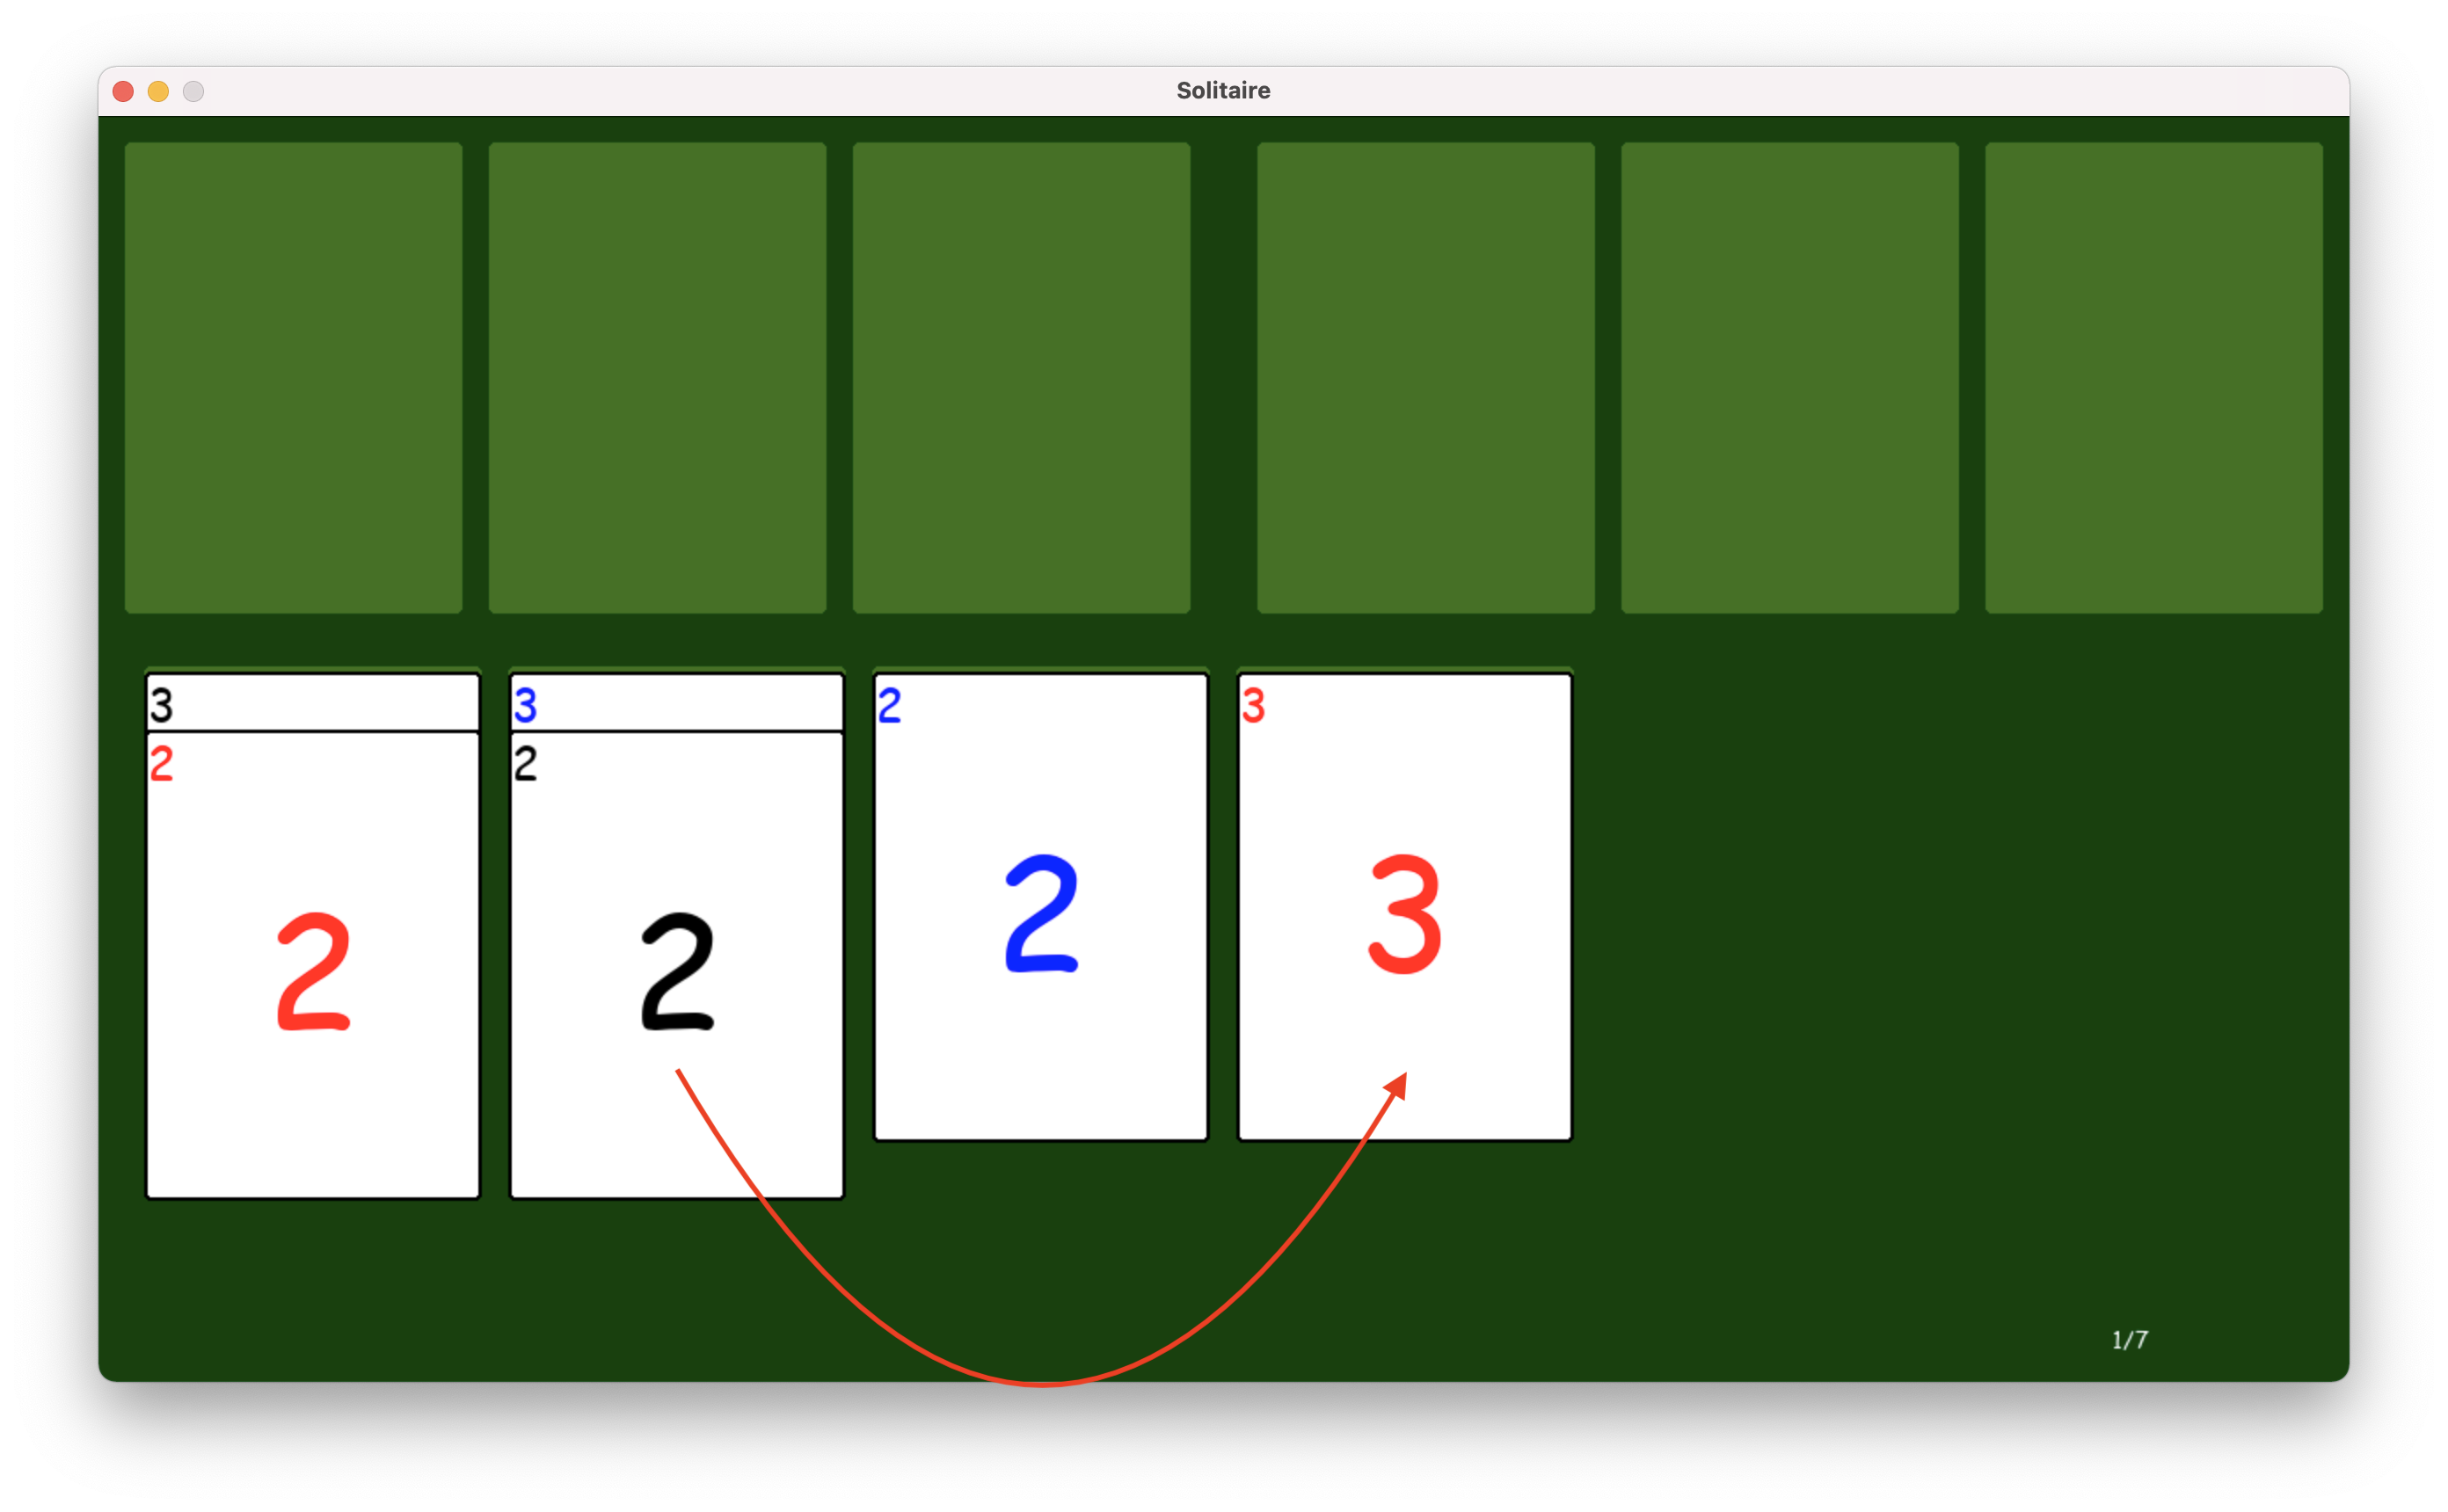
\includegraphics[scale=0.25]{problem_4.png}
    		\caption{перемещение черной двойки на красную тройку}
    	\end{center}
\end{figure}
\begin{figure}[H]
    	\begin{center}
    		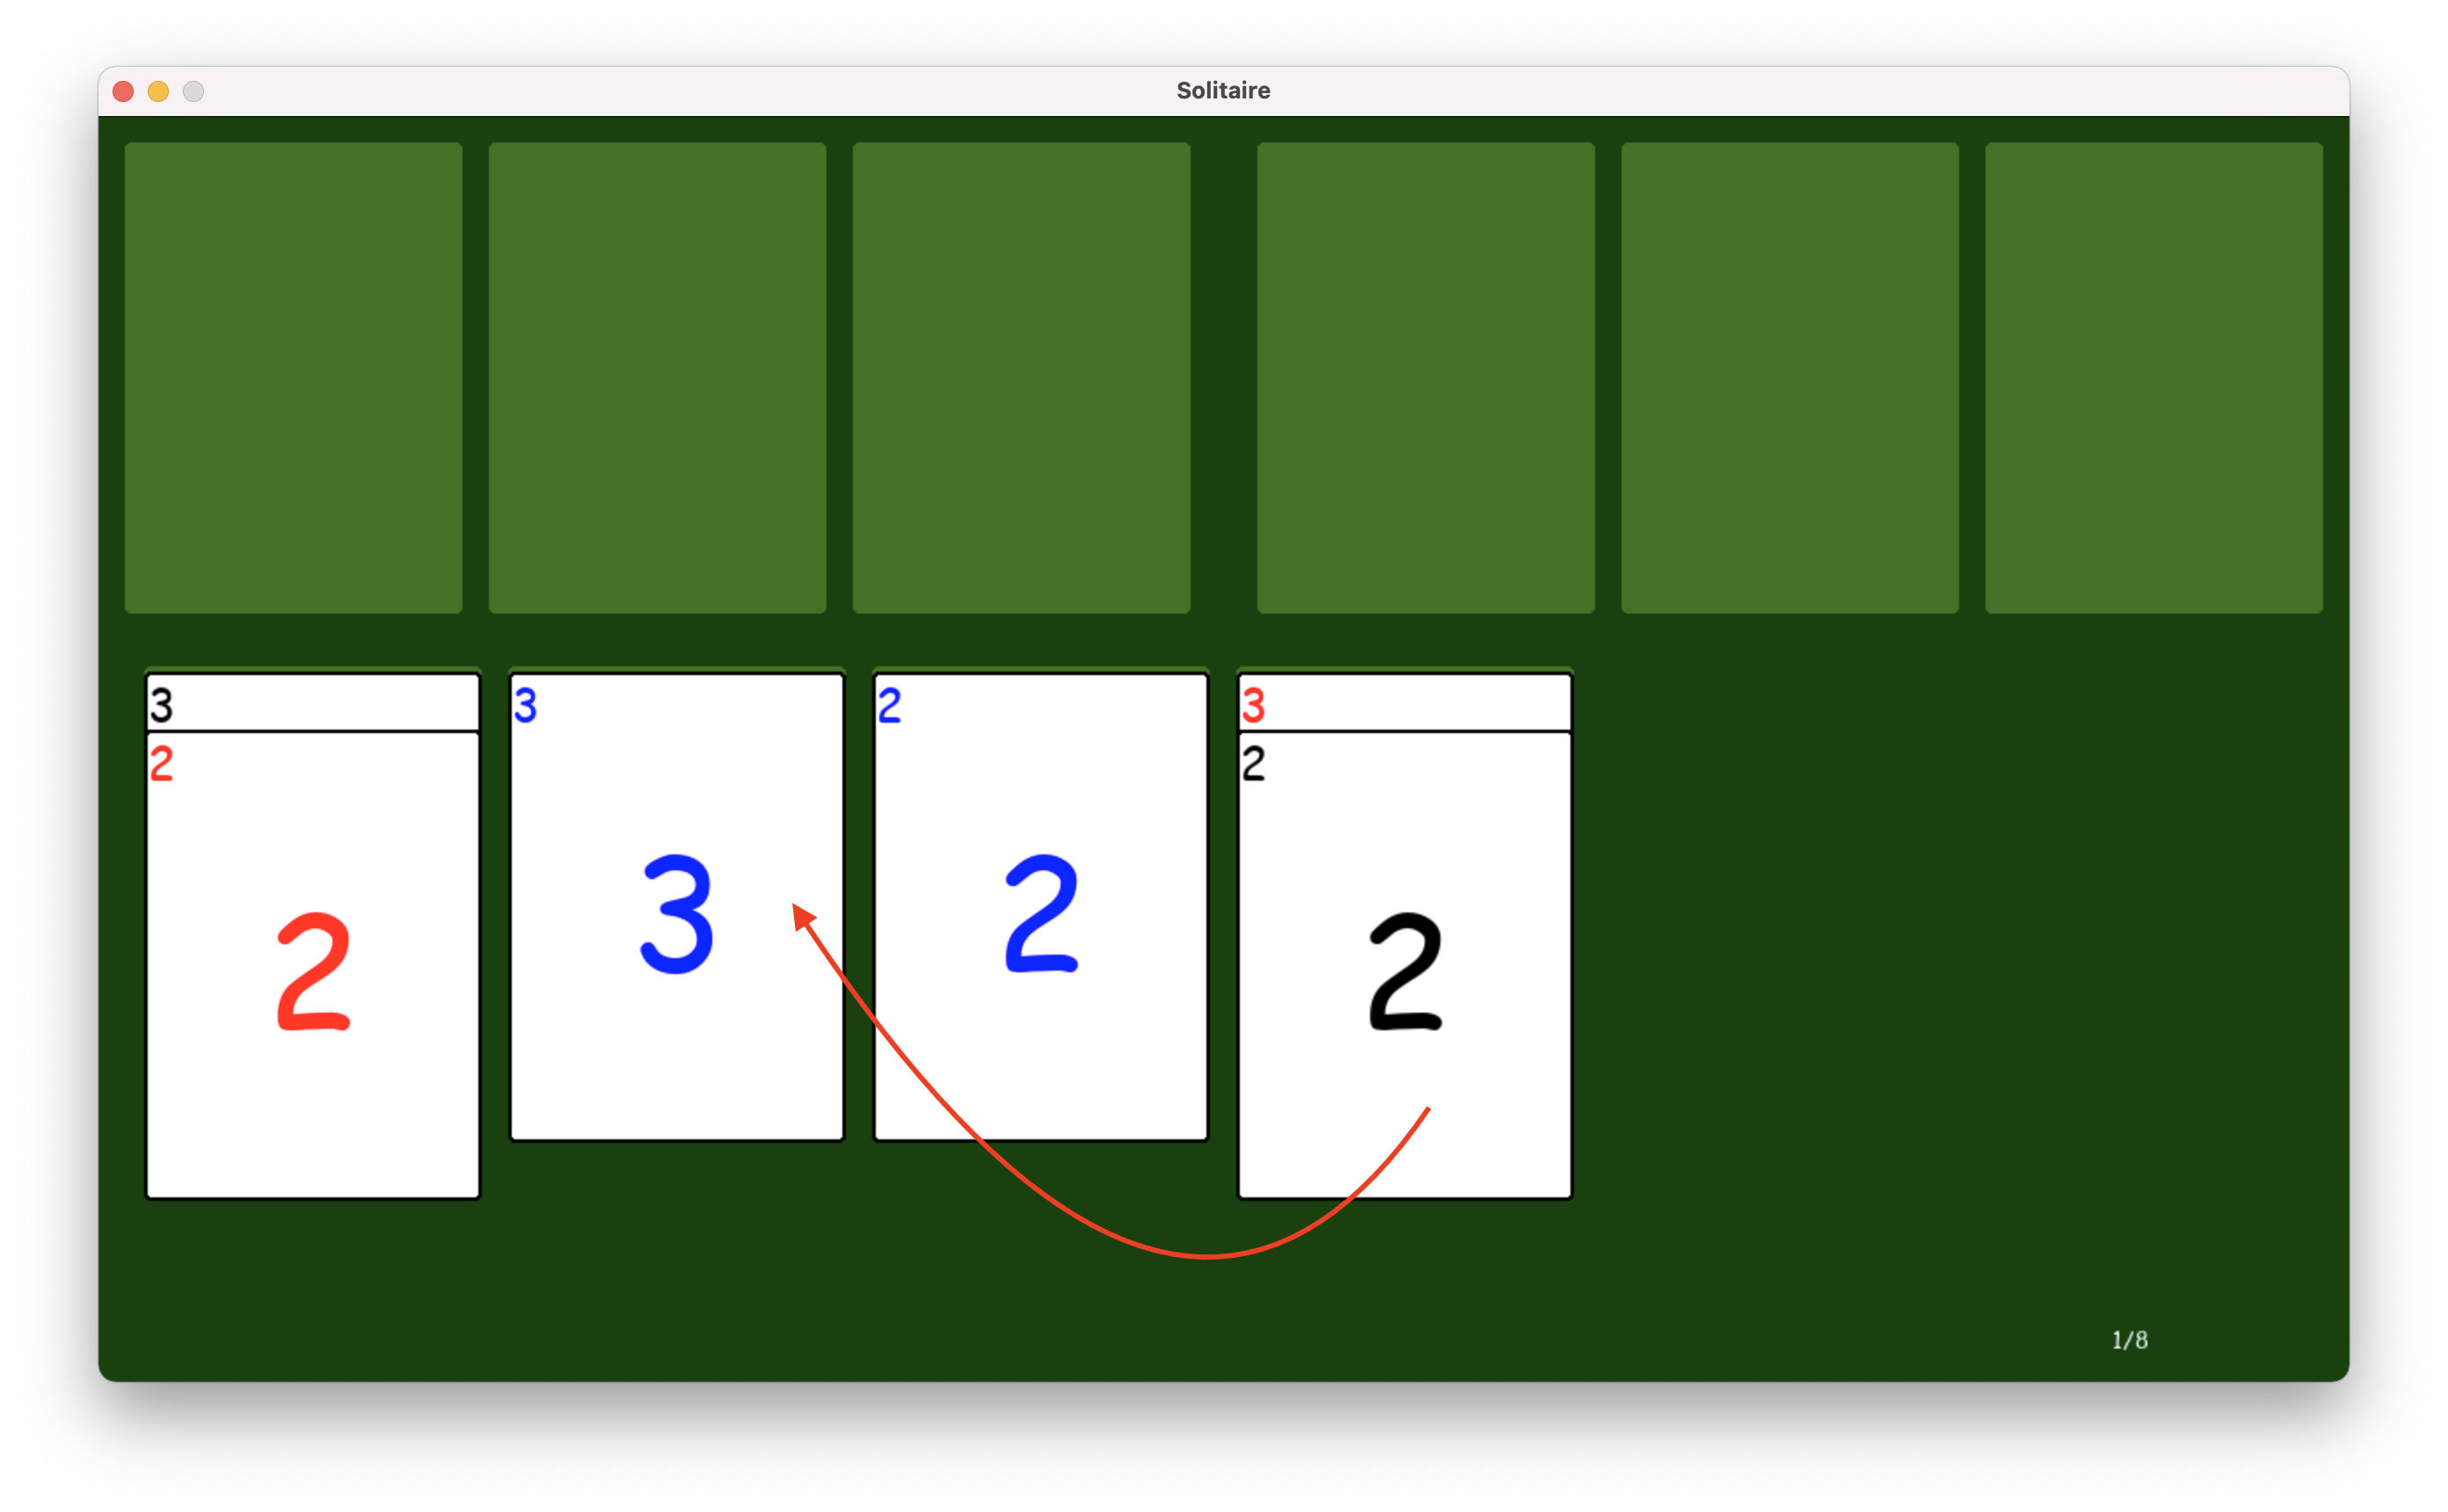
\includegraphics[scale=0.25]{problem_3.png}
    		\caption{перемещение черной двойки на синюю тройку}
    	\end{center}
\end{figure}

Благодаря хранению множества возможных к снятию карт, получилось решить данную проблему и оптимизировать решение.
На рисунках 3.5-3.6 представлен пример состояний, которые наша система считает идентичными.
\begin{figure}[H]
    	\begin{center}
    		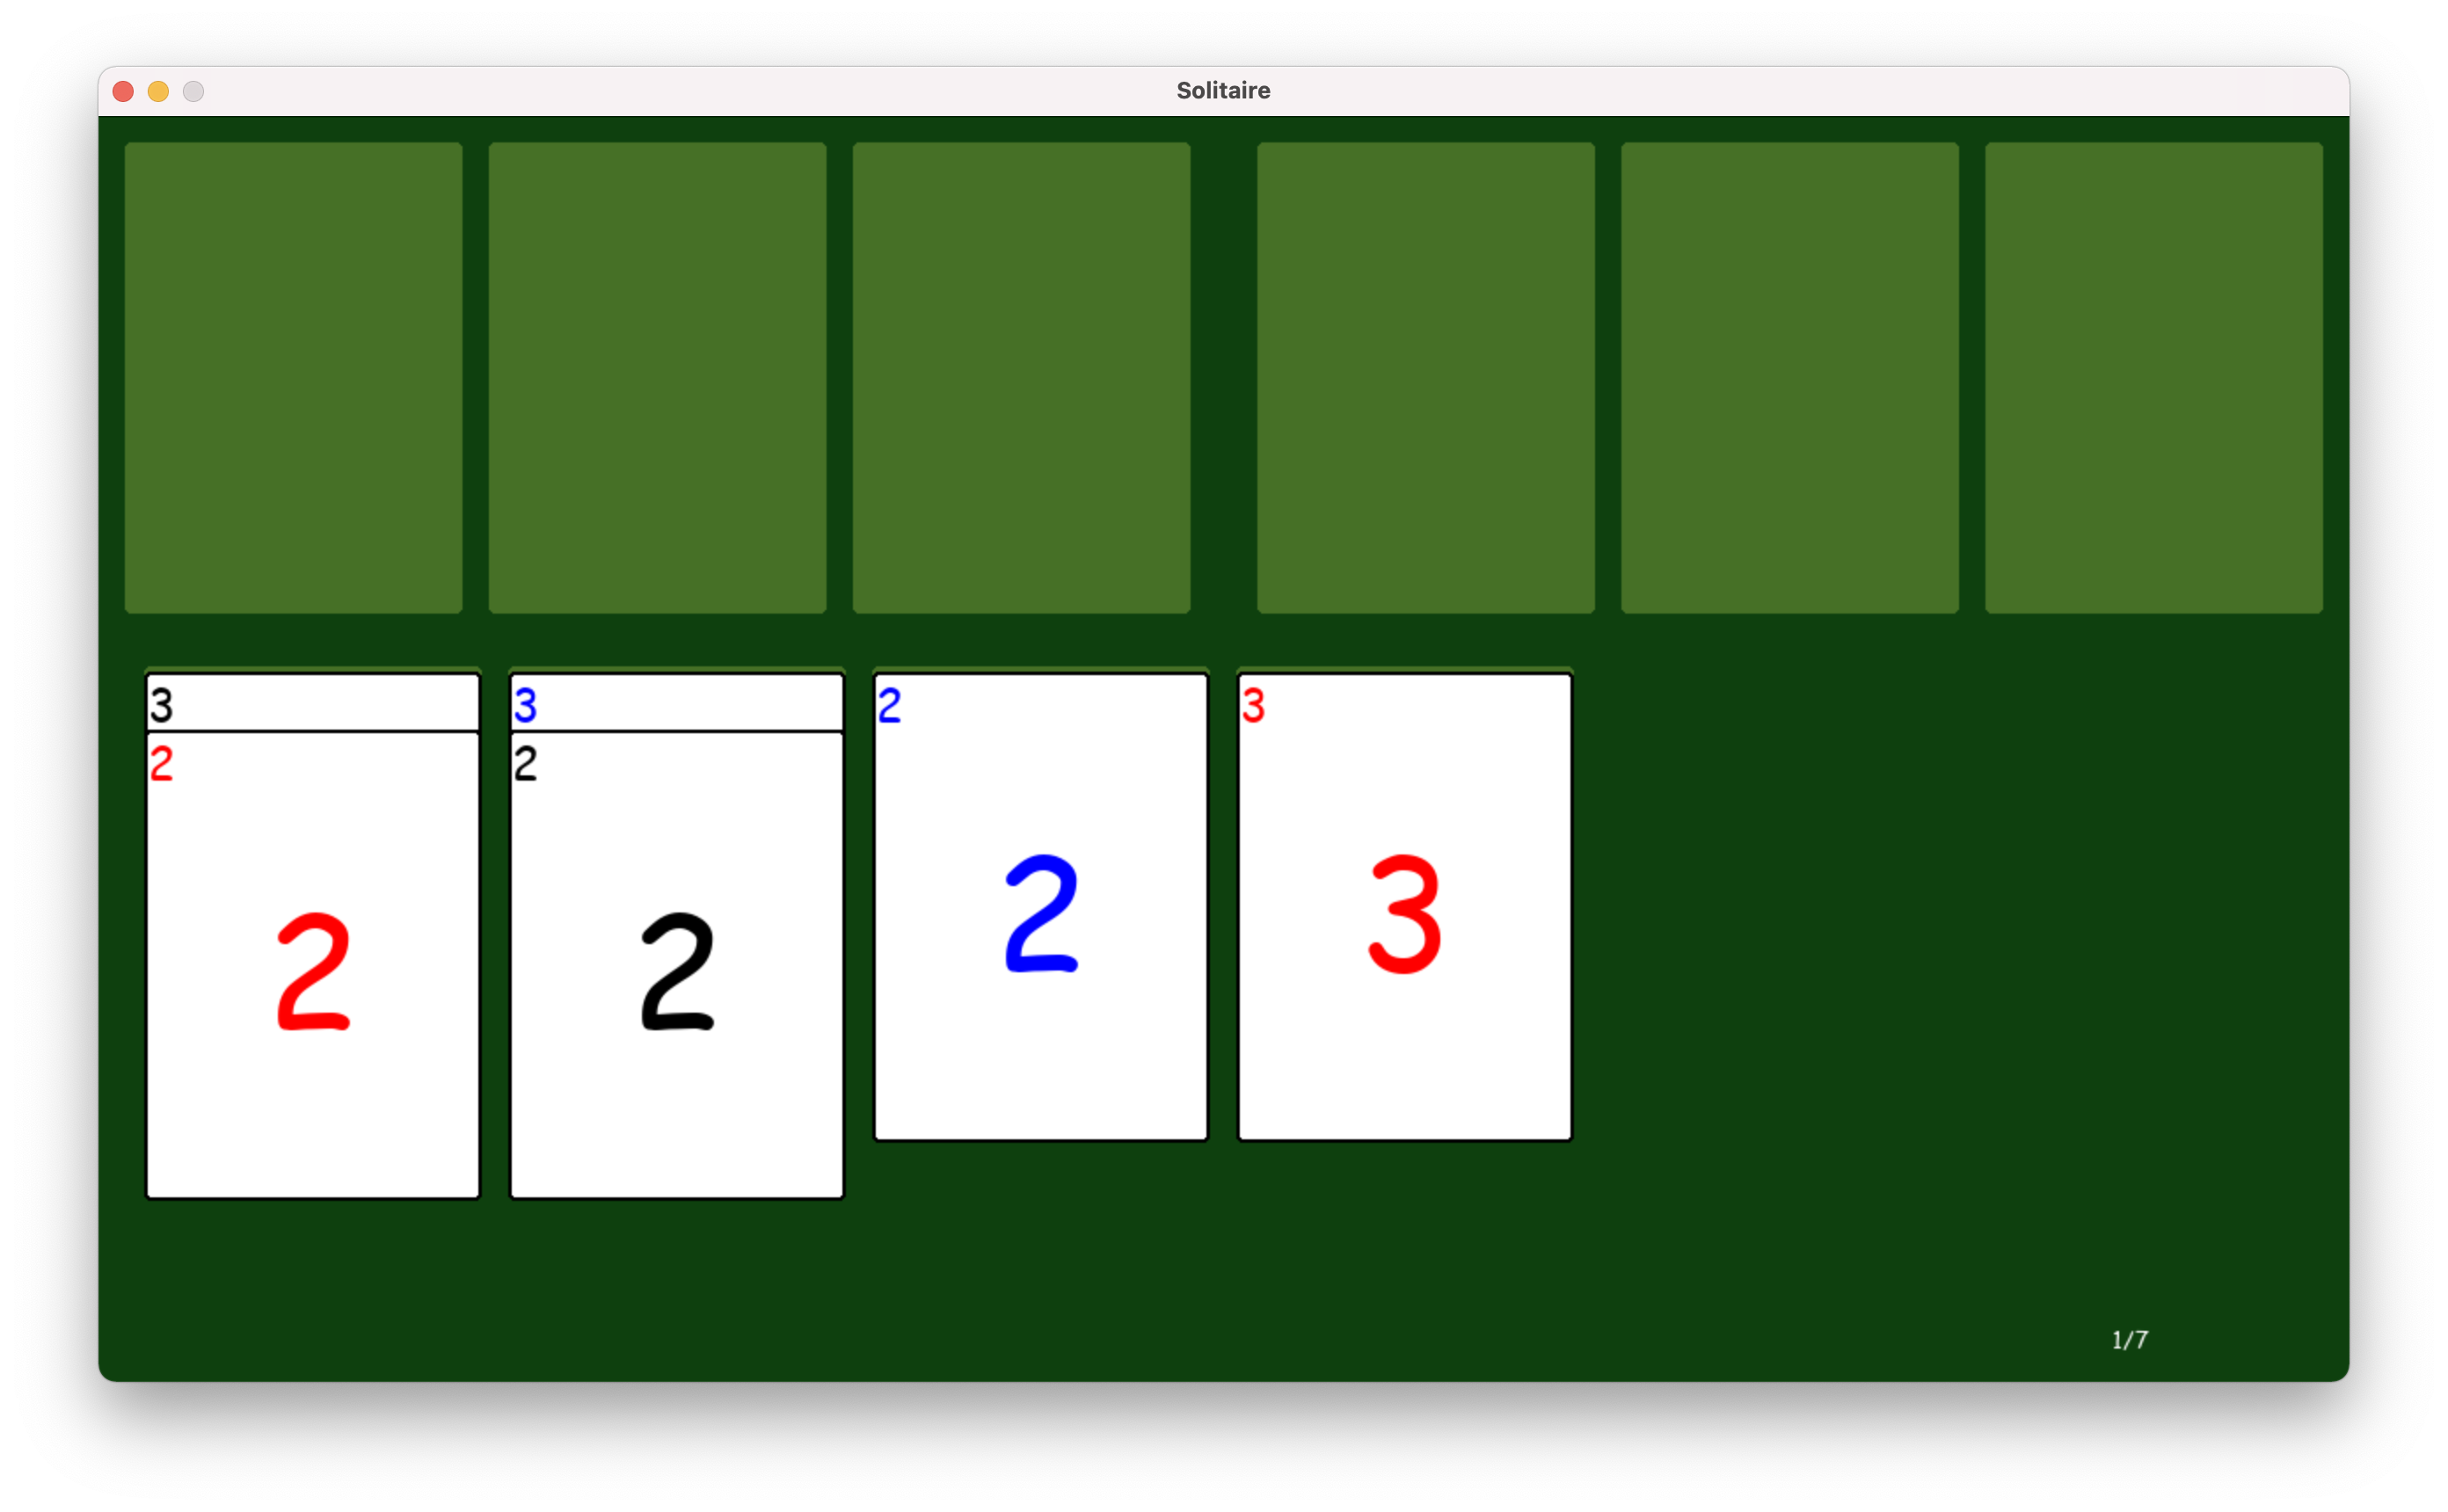
\includegraphics[scale=0.25]{problem_10.png}
    		\caption{перемещение синей двойки на красную тройку}
    	\end{center}
\end{figure}
\begin{figure}[H]
    	\begin{center}
    		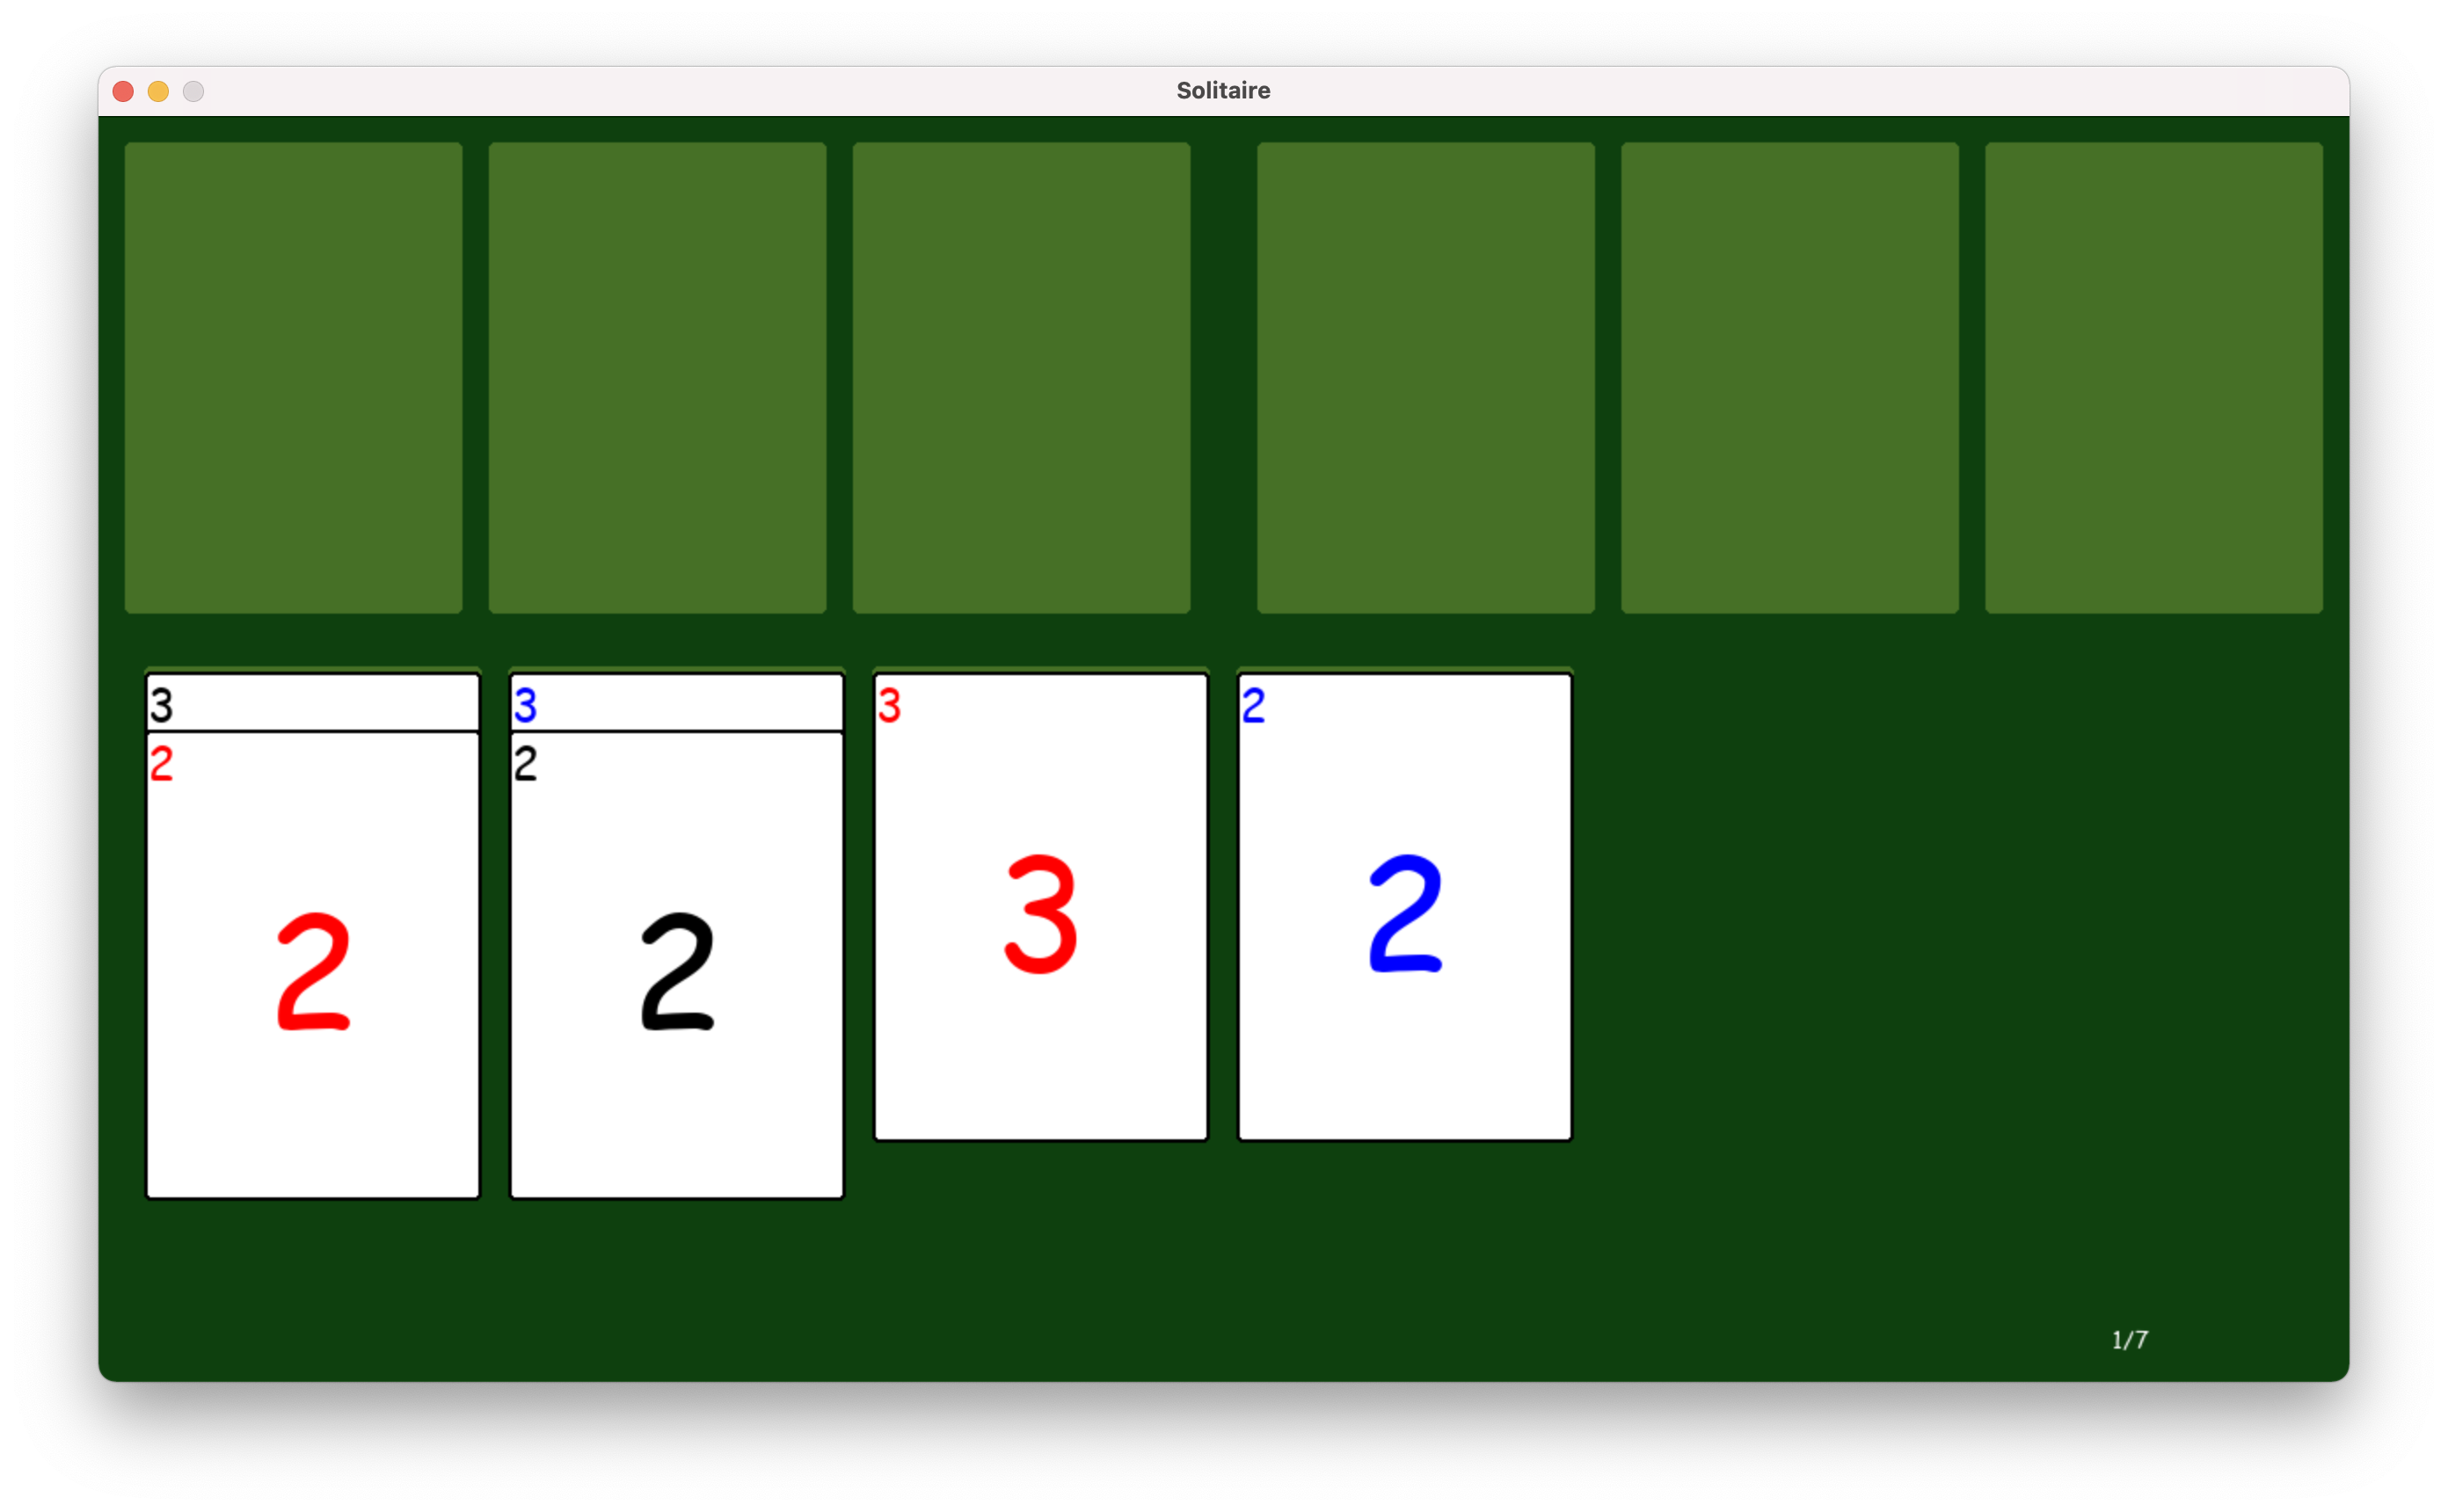
\includegraphics[scale=0.25]{problem_11.png}
    		\caption{перемещение синей двойки на красную тройку}
    	\end{center}
\end{figure}

\chapter{IDEF0}
На рисунках 4.1-4.3 представлена IDEF0 диаграмма решения:

\begin{figure}[H]
    	\begin{center}
    		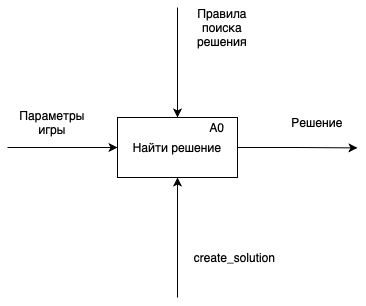
\includegraphics[scale=1]{idef_1.png}
    		\caption{IDEF0 A0}
    	\end{center}
\end{figure}

\begin{figure}[H]
    	\begin{center}
    		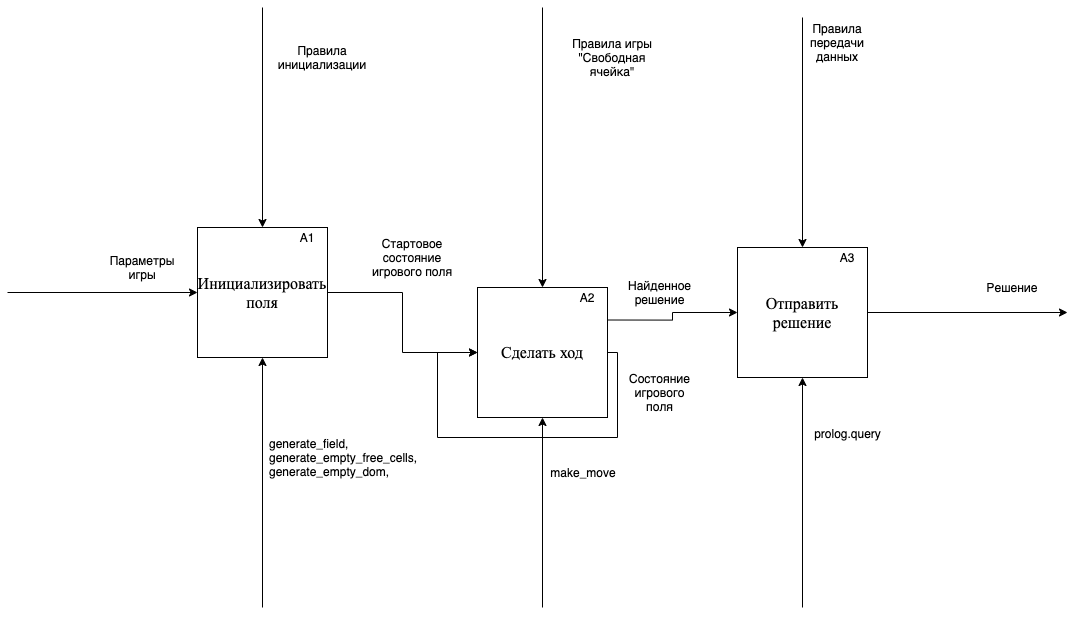
\includegraphics[scale=0.45]{idef_2.png}
    		\caption{IDEF0 A1-A3}
    	\end{center}
\end{figure}

\begin{figure}[H]
    	\begin{center}
    		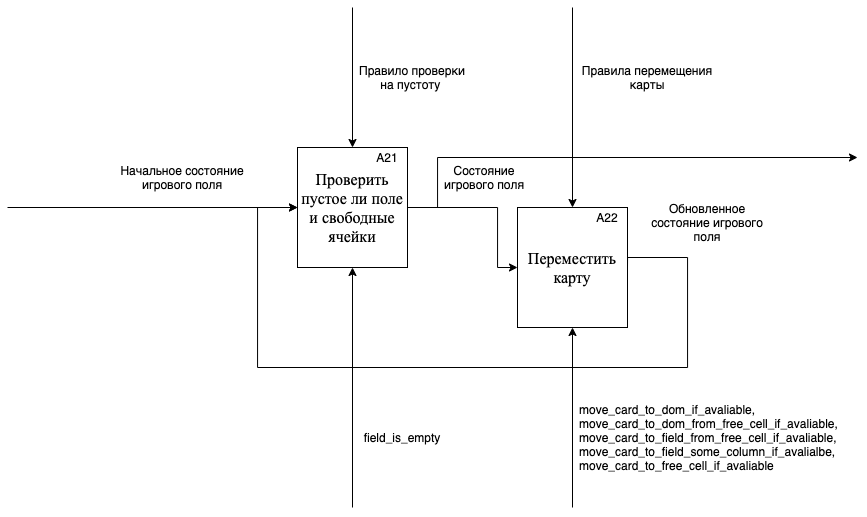
\includegraphics[scale=0.45]{idef_3.png}
    		\caption{IDEF0 A11-A12}
    	\end{center}
\end{figure}

\chapter{Описание правил}
В данном разделе описаны все правила, переменные, приведены примеры использования данных правил.
\section{solve}
Правило, с которого начинается работа программы. На основе MaxValue и ColorsCount определяются количество свободных ячеек, размеры поля и дома. Генерируются поле, пустые свободные ячейки и дом. Создаётся переменная State для хранения состояний. В конце проверяется правило, отвечающее за поиск решения.

Переменные:
\begin{itemize}

\item MaxValue – хранит количество карт каждого цвета;
\item ColorsCount – хранит количество цветов карт;
\item Solution – переменная, которая в результате работы программы получает набор состояний, являющийся последовательным решением задачи;
\item States – переменная, для хранения набора состояний;
\item Dom – переменная, в которой хранятся значения карт, находящихся в доме;
\item FreeCells – переменная, в которой хранятся значения карт, находящихся в свободных ячейках;
\item Field – переменная, в которой хранится набор карт, находящихся на поле;
\item FreeCellsSize – хранит размер переменной FreeCells, то есть количество свободных ячеек в игре;
\item ReservedCellsCount – хранит количество занятых свободных ячеек;
\item NumberOfColumns – хранит количество столбцов игрового поля Field.
\end{itemize}

В листинге 5.1 представлена реализация правила solve

\begin{lstlisting}[label=some-code, caption=реализация правила solve]
solve(MaxValue, ColorsCount, Solution) :-
	FreeCellsSize is ColorsCount,
	ReservedCellsCount is 0,
	NumberOfColumns is ColorsCount * 2,
	generate_field(MaxValue, ColorsCount, Field),
	generate_empty_free_cells(FreeCells),
	generate_empty_dom(ColorsCount, Dom),
	stm_init(State),
	stm_append_value_if_not_in_stm(State, [Dom, FreeCells, Field], States),
	make_move(Field, MaxValue, NumberOfColumns, FreeCells, Dom, FreeCellsSize, ReservedCellsCount, States, Solution).
\end{lstlisting}

В листинге 5.2 представлен пример работы правила solve
\begin{lstlisting}[caption=пример работы правила solve]
?- solve(4, 2, Solution).
Solution = [[[[[0,0],[1,0]],[[0,1],[1,1]]],[],[[],[],[],[]]],
[[[[0,0],[1,0]],[[1,1]]],[],[[[0,1]],[],[],[]]],
[[[[0,0],[1,0]],[]],[],[[[0,1]],[],[],[[1,1]]]],
[[[[1,0]],[]],[],[[[0,1]],[],[[0,0]],[[1,1]]]],
[[[],[]],[],[[[0,1]],[[1,0]],[[0,0]],[[1,1]]]]].
\end{lstlisting}
\section{make\_move}
make\_move – это набор из шести равноценных правил, пять из которых проверяет возможность совершения одного из ходов в игре: положить карту из поля в дом, из свободных ячеек в дом, из свободных ячеек в поле, из поля в свободные ячейки и переложить карту между столбцами поля. Первое правило нужно для передачи результата в переменную Solution и завершения поиска решения. Если поле и свободные ячейки пусты, переменная Solution успешно унифицируется с переменной, хранящей набор состояний. В остальных правилах сначала создается переменная Card, хранящая значение одной карты, затем, в зависимости от правила, идёт проверка условий и совершение хода данного типа. Если данный набор состояний получен в первый раз, он добавляется в переменную NSSnapshot. В конце снова проверяется правило make\_move, но уже с новыми значениями переменных.

Переменные:
\begin{itemize}
\item Field – переменная, в которой хранится набор карт, находящихся на поле;
\item MaxValue – хранит количество карт каждого цвета;
\item NumberOfColumns – хранит количество столбцов поля Field;
\item FreeCells – переменная, в которой хранятся значения карт, находящихся в свободных ячейках;
\item Dom – переменная, в которой хранятся значения карт, находящихся в доме;
\item FreeCellsSize – хранит размер переменной FreeCells, то есть количество свободных ячеек в игре;
\item ReservedCellsCount – хранит количество занятых свободных ячеек;
\item Snapshots – переменная, для хранения набора состояний;
\item Solution – переменная, которая в результате работы программы получает набор состояний, являющийся последовательным решением задачи;
\item Card – переменная для хранения значения одной карты;
\item RowOfCard – переменная хранит длину столбца, наверху которого находится Card;
\item FieldResult – переменная, в которой хранится набор карт, находящихся на поле, после совершения хода;
\item DomResult – переменная, в которой хранятся значения карт, находящихся в доме, после совершения хода;
\item FreeCellsResult – переменная, в которой хранятся значения карт, находящихся в свободных ячейках, после совершения хода;
\item ReservedFreeCellsCountResult – переменная хранит количество занятых свободных ячеек, после совершения хода;
\item NSSnapshot(Next Step Snapshot) – переменная, в которой хранится обновленный набор состояний, после совершения хода.
\end{itemize}

В листинге 5.3 представлена реализация make\_move

\begin{lstlisting}[label=some-code, caption=реализация make\_move]
make_move(Field, _, _, _, _, _, 0, Solution, Solution) :-
	field_is_empty(Field), !.

make_move(Field, MaxValue, NumberOfColumns, FreeCells, Dom, FreeCellsSize, ReservedFreeCells, Snapshots, Solution) :-
	get_top_card(Field, Card, RowOfCard),
	move_card_to_dom_if_avaliable(Card, Field, RowOfCard, Dom, MaxValue, FieldResult, DomResult),
	stm_append_value_if_not_in_stm(Snapshots, [DomResult, FreeCells, FieldResult], NSSnapshot),
	make_move(FieldResult, MaxValue, NumberOfColumns, FreeCells, DomResult, FreeCellsSize, ReservedFreeCells, NSSnapshot, Solution), !.

make_move(Field, MaxValue, NumberOfColumns, FreeCells, Dom, FreeCellsSize, ReservedFreeCells, Snapshots, Solution) :-
	process_free_cell_card(FreeCells, Card),
	move_card_to_dom_from_free_cell_if_avaliable(Card, Dom, FreeCells, ReservedFreeCells, DomResult, FreeCellsResult, ReservedFreeCellsCountResult, MaxValue),
	stm_append_value_if_not_in_stm(Snapshots, [DomResult, FreeCellsResult, Field], NSSnapshot),
	make_move(Field, MaxValue, NumberOfColumns, FreeCellsResult, DomResult, FreeCellsSize, ReservedFreeCellsCountResult, NSSnapshot, Solution), !.

make_move(Field, MaxValue, NumberOfColumns, FreeCells, Dom, FreeCellsSize, ReservedFreeCells, Snapshots, Solution) :-
	process_free_cell_card(FreeCells, Card),
	move_card_to_field_from_free_cell_if_avaliable(Card, Field, FreeCells, NumberOfColumns, ReservedFreeCells, FieldResult, FreeCellsResult, ReservedFreeCellsCountResult),
	stm_append_value_if_not_in_stm(Snapshots, [Dom, FreeCellsResult, FieldResult], NSSnapshot),
	make_move(FieldResult, MaxValue, NumberOfColumns, FreeCellsResult, Dom, FreeCellsSize, ReservedFreeCellsCountResult, NSSnapshot, Solution), !.

make_move(Field, MaxValue, NumberOfColumns, FreeCells, Dom, FreeCellsSize, ReservedFreeCells, Snapshots, Solution) :-
	get_top_card(Field, _, RowOfCard),
	move_card_to_field_some_column_if_avalialbe(Field, NumberOfColumns, RowOfCard, FieldResult),
	stm_append_value_if_not_in_stm(Snapshots, [Dom, FreeCells, FieldResult], NSSnapshot),
	make_move(FieldResult, MaxValue, NumberOfColumns, FreeCells, Dom, FreeCellsSize, ReservedFreeCells, NSSnapshot, Solution), !.

make_move(Field, MaxValue, NumberOfColumns, FreeCells, Dom, FreeCellsSize, ReservedFreeCells, Snapshots, Solution) :-
	get_top_card(Field, Card, RowOfCard),
	move_card_to_free_cell_if_avaliable(Card, RowOfCard, Field, FreeCells, FreeCellsSize, ReservedFreeCells, FieldResult, FreeCellsResult, ReservedCellsCountResult),
	stm_append_value_if_not_in_stm(Snapshots, [Dom, FreeCellsResult, FieldResult], NSSnapshot),
	make_move(FieldResult, MaxValue, NumberOfColumns, FreeCellsResult, Dom, FreeCellsSize, ReservedCellsCountResult, NSSnapshot, Solution), !.

\end{lstlisting}

В листинге 5.4 представлен пример работы правила make\_move
\begin{lstlisting}[caption=пример работы правила make\_move]
?- make_move([[[0, 0], [2, 1]],
[[2, 0], [3, 0]],
[[1, 1], [3, 1]],
[[1, 0], [0, 1]]],
          4, 2,
          [],
          [[],[]],
          2, 0, [], Solution)

Solution = [[[[[2, 1], [1, 1], [0, 1], [3, 1]], [[2, 0], [1, 0], [0, 0], [3, 0]]], [], [[], [], [], []]], [[[[2, 1], [1, 1], [0, 1], [3, 1]], [[1, 0], [0, 0], [3, 0]]], [[2, 0]], [[], [], [], []]], [[[[2, 1], [1, 1], [0, 1], [3, 1]], [[0, 0], [3, 0]]], [[1, 0], [2, 0]], [[], [], [], []]], [[[[2, 1], [1, 1], [0, 1], [3, 1]], [[3, 0]]], [[1, 0], [2, 0]], [[[0, 0]], [], [], []]], [[[[2, 1], [1, 1], [0, 1], [3, 1]], []], [[1, 0], [2, 0]], [[[0, 0]], [[3, 0]], [], []]], [[[[2, 1], [1, 1], [0, 1], [3, 1]], []], [[1, 0]], [[[0, 0]], [[2, 0], [3, 0]], [], []]], [[[[2, 1], [1, 1], [0, 1], [3, 1]], []], [[0, 0], [1, 0]], [[], [[2, 0], [3, 0]], [], []]], [[[[2, 1], [1, 1], [0, 1], [3, 1]], []], [[0, 0]], [[[1, 0]], [[2, 0], [3, 0]], [], []]], [[[[1, 1], [0, 1], [3, 1]], []], [[2, 1], [0, 0]], [[[1, 0]], [[2, 0], [3, 0]], [], []]], [[[[0, 1], [3, 1]], []], [[2, 1], [0, 0]], [[[1, 0]], [[1, 1], [2, 0], [3, 0]], [], []]], [[[[0, 1], [3, 1]], []], [[2, 1]], [[[1, 0]], [[0, 0], [1, 1], [2, 0], [3, 0]], [], []]], [[[[0, 1], [3, 1]], []], [[1, 0], [2, 1]], [[], [[0, 0], [1, 1], [2, 0], [3, 0]], [], []]], [[[[0, 1], [3, 1]], []], [[1, 0]], [[[2, 1]], [[0, 0], [1, 1], [2, 0], [3, 0]], [], []]], [[[[0, 1], [3, 1]], []], [], [[[1, 0], [2, 1]], [[0, 0], [1, 1], [2, 0], [3, 0]], [], []]], [[[[3, 1]], []], [], [[[1, 0], [2, 1]], [[0, 0], [1, 1], [2, 0], [3, 0]], [], [[0, 1]]]], [[[[3, 1]], []], [], [[[2, 1]], [[0, 0], [1, 1], [2, 0], [3, 0]], [], [[1, 0], [0, 1]]]], [[[[3, 1]], []], [], [[[0, 0], [2, 1]], [[1, 1], [2, 0], [3, 0]], [], [[1, 0], [0, 1]]]], [[[], []], [], [[[0, 0], [2, 1]], [[1, 1], [2, 0], [3, 0]], [[3, 1]], [[1, 0], [0, 1]]]]]
\end{lstlisting}
\section{is\_equal\_sets}
Правило проверяет эквивалентность двух списков List1 и List2, предварительно переведя их в множества Set1 и Set2 соответственно, после сортирует полученные множества и сохраняет результат в переменные SortedSet1 и SortedSet2 соответственно. Полученные отсортированные множества сравниваются на эквивалентность.

Переменные:
\begin{itemize}
\item List1 – список 1;
\item List2 – список 2;
\item Set1 – переменная, в которой хранится List1 без дубликатов значений;
\item Set2 – переменная, в которой хранится List2 без дубликатов значений;
\item SortedSet1 – переменная, в которой хранится отсортированная версия Set1;
\item SortedSet2 – переменная, в которой хранится отсортированная версия Set2.
\end{itemize}

В листинге 5.5 представлена реализация правила is\_equal\_sets

\begin{lstlisting}[label=some-code, caption=реализация правила is\_equal\_sets]
is_equal_sets(List1, List2) :-
	list_to_set(List1, Set1),
	list_to_set(List2, Set2),
	sort(Set1, SortedSet1),
	sort(Set2, SortedSet2),
	is_equal(SortedSet1, SortedSet2).
\end{lstlisting}
В листинге 5.6 представлены примеры работ правила is\_equal\_sets

\begin{lstlisting}[label=some-code, caption=примеры работ правила is\_equal\_sets]
?- is_equal_sets([1,3,2,3,5],[3,1,2,5]).
true

?- is_equal_sets([1,3,2,3,2],[3,9,2,4]).
false
\end{lstlisting}
\section{insert}
Этот набор равноценных правил используется для добавления в хвост списка значения переменной Value.

Переменные:
\begin{itemize}
\item Value – переменная, значение которой помещается в хвост списка;
\item H – переменная, обозначающая голову списка;
\item T, T2 – переменные, обозначающие хвост списка.
\end{itemize}

В листинге 5.7 представлена реализация правила insert

\begin{lstlisting}[label=some-code, caption=реализация правила insert]
insert([H | T], [H | T2], Value) :-
	insert(T, T2, Value), !.

insert([H | []], [H, Value], Value) :- !.

insert([], [Value], Value) :- !.
\end{lstlisting}

В листинге 5.8 представлен пример работы правила insert

\begin{lstlisting}[label=some-code, caption=пример работы правила insert]
?- insert([1,2,3],Result, 4)
Result = [1,2,3,4]
\end{lstlisting}
\section{insert\_to\_head}
Этот набор равноценных правил используется для добавления в голову списка значения переменной Element.

Переменные:
\begin{itemize}
\item Element – переменная, значение которой помещается в хвост списка;
\item H – переменная, обозначающая голову списка;
\item T, T2 – переменные, обозначающие хвост списка.
\end{itemize}

В листинге 5.9 представлена реализация правила insert\_to\_head

\begin{lstlisting}[label=some-code, caption=реализация правила insert\_to\_head]
insert_to_head([H | T], Element, [Element, H | T]) :- !.

insert_to_head([], Element, [Element]).
\end{lstlisting}
В листинге 5.10 представлен пример работы правила insert\_to\_head

\begin{lstlisting}[label=some-code, caption=пример работы правила insert\_to\_head]
insert_to_head([1,2,3],4, Result)
Result = [4, 1, 2, 3]
\end{lstlisting}

\section{set\_value}
Правило задаёт значение переменной.

В листинге 5.11 представлена реализация правила set\_value

\begin{lstlisting}[label=some-code, caption=реализация правила set\_value]
set_value(Hardcode, Hardcode).
\end{lstlisting}

В листинге 5.12 представлен пример работы правила set\_value

\begin{lstlisting}[label=some-code, caption=пример работы правила set\_value]
set_value(X, 12)
X = 12
\end{lstlisting}

\section{is\_equal}
Правило используется для проверки эквивалентности значений двух переменных.

В листинге 5.13 представлена реализация правила is\_equal

\begin{lstlisting}[label=some-code, caption=реализация правила is\_equal]
is_equal(Value, Value).
\end{lstlisting}
В листинге 5.14 представлен пример работы правила is\_equal

\begin{lstlisting}[label=some-code, caption=пример работы правила is\_equal]
is_equal(12,12)
true

is_equal(12,13)
false
\end{lstlisting}

\section{is\_not\_equal}
Правило используется для проверки того, что значения переменных не эквивалентны.
В листинге 5.15 представлена реализация правила is\_not\_equal

\begin{lstlisting}[label=some-code, caption=реализация правила is\_not\_equal]
is_not_equal(Value, Value) :- !, false.

is_not_equal(_, _).
\end{lstlisting}
В листинге 5.16 представлены примеры работы  правила is\_not\_equal

\begin{lstlisting}[label=some-code, caption=пример работы правила is\_not\_equal]
is_not_equal(12,12)
false

is_not_equal(12,13)
true
\end{lstlisting}

\section{delete\_nth\_element\_from\_list}
Правило используется для удаления N-ого элемента списка List, результат сохраняется в переменной ResultList. 

Главное правило delete\_nth\_element\_from\_list использует рекурсивную версию правила с приставкой \_internal. Внутреннее правило двигается по списку и передаёт значение головы списка списку ResultList. Как только количество итераций будет равно значению переменной N, списку ResultList будет передан оставшийся хвост начального списка без N-ого элемента, после чего дальнейшая проверка правила будет прервана.

Переменные:
\begin{itemize}
\item List – начальный список, из которого удаляют элемент;
\item N – номер позиции в списке элемента, который нужно удалить;
\item ResultList – список-результат, без n-ого элемента.
\end{itemize}

В листинге 5.17 представлена реализация правила

delete\_nth\_element\_from\_list

\begin{lstlisting}[label=some-code, caption=реализация правила delete\_nth\_element\_from\_list]
delete_nth_element_from_list(List, N, ResultList) :-
	delete_nth_element_from_list_internal(List, N, ResultList, 0).

delete_nth_element_from_list_internal([_ | T], Iteration, T, Iteration) :- !.

delete_nth_element_from_list_internal([H | T1], N, [H | T2], Iteration) :-
	NSIteration is Iteration + 1,
	delete_nth_element_from_list_internal(T1, N, T2, NSIteration).

\end{lstlisting}
В листинге 5.18 представлен пример работы 

правила delete\_nth\_element\_from\_list

\begin{lstlisting}[label=some-code, caption=пример работы правила delete\_nth\_element\_from\_list]
delete_nth_element_from_list([1,2,3],1,Res)
Res = [1, 3]
\end{lstlisting}

\section{get\_element}
Правило позволяет получить определенный элемент списка по его индексу. Используется правило nth0, которое позволяет получить значение элемента по индексу.

Переменные:
\begin{itemize}
\item List – переменная, хранящая список;
\item Index – переменная, хранящая индекс элемента, который нужно получить;
\item Element – переменная, в которой сохраняется значение нужного элемента списка.
\end{itemize}

В листинге 5.19 представлена реализация правила get\_element

\begin{lstlisting}[label=some-code, caption=реализация правила get\_element]
get_element(List, Index, Element) :-
   nth0(Index, List, Element).

get_element([], _, []).

get_element(_, _, []).

\end{lstlisting}
В листинге 5.20 представлен пример работы правила get\_element

\begin{lstlisting}[label=some-code, caption= пример работы  правила get\_element]
get_element([1,2,3,4,5],2,Res)
Res = 3
\end{lstlisting}
\section{get\_element\_with\_len}
Правило возвращает элемент списка и его длину. Здесь также, как и в правиле get\_element, используется правило nth0, после чего используется правило length для получения длинны списка, хранящегося в переменной Element.

Переменные:
\begin{itemize}
\item List – переменная, хранящая список;
\item Index – переменная, хранящая индекс элемента, который нужно получить;
\item Element – переменная, в которой сохраняется значение нужного элемента списка;
\item Len – переменная для хранения длины списка Element.
\end{itemize}

В листинге 5.21 представлена реализация правила get\_element\_with\_len

\begin{lstlisting}[label=some-code, caption=реализация правила get\_element\_with\_len]
get_element_with_len(List, Index, Element, Len) :-
	nth0(Index, List, Element),
	length(Element, Len).

get_element_with_len([], _, [], _).

get_element_with_len(_, _, [], _).

\end{lstlisting}

В листинге 5.22 представлен пример работы правила get\_element\_with\_len

\begin{lstlisting}[label=some-code, caption=пример работы правила get\_element\_with\_len]
get_element_with_len([[1,2],[1,2,3],[1,2,3,4,5]],2,Res,ResLen)
Res = [1, 2, 3, 4, 5], ResLen = 5
\end{lstlisting}

\section{cnt\_mod}
Переменная Res принимает значение остатка от деления переменной A на переменную B.

Переменные:
\begin{itemize}
\item A, B – численные переменные;
\item Res – переменная, в которой сохраняется результат.
\end{itemize}

В листинге 5.23 представлена реализация правила cnt\_mod

\begin{lstlisting}[label=some-code, caption=реализация правила cnt\_mod]
cnt_mod(A, B, Res) :-
	Res is A mod B.
\end{lstlisting}
В листинге 5.24 представлен пример работы реализация правила cnt\_mod

\begin{lstlisting}[label=some-code, caption=пример работы правила cnt\_mod]
cnt_mod(6,3, Res)
Res = 0

cnt_mod(6,4, Res)
Res = 2
\end{lstlisting}

\section{replace}
Правило используется для того, чтобы менять значение элемента списка под номером Index на значение переменной Element. Если Index больше длины списка, значение переменной Element будет вставлено в хвост списка.

Переменные:
\begin{itemize}
\item List – переменная, хранящая список;
\item Index – переменная, хранящая индекс элемента, который нужно заменить;
\item Element – переменная хранящая значение, которое нужно поместить в список;
\item Res – переменная возвращающая результат работы правила.
\end{itemize}

В листинге 5.25 представлена реализация правила replace

\begin{lstlisting}[label=some-code, caption=реализация правила replace]
replace(Index, List, Element, Result) :-
  nth0(Index, List, _, Res),
  nth0(Index, Result, Element, Res), !.

replace(Index, List, Element, Res) :-
	length(List, ListLength),
	Index >= ListLength,
	insert(List, Res, Element).
\end{lstlisting}
В листинге 5.26 представлен пример работы реализация правила replace

\begin{lstlisting}[label=some-code, caption=реализация правила replace]
replace(1, [1,2,3,4,5], 9, Result)
Result = [1, 9, 3, 4, 5]
\end{lstlisting}

\section{state\_inside\_state\_machine}
Правило используется для проверки того находится ли данное [Dom, FreeCells, Field] состояние в наборе или нет. Дом и свободные ячейки проверяются по совпадению с значениями сохраненными в наборе. В поле же проверяются не все элементы, а лишь набор карт, доступных к снятию во всех столбцах. На основе списка этих карт с помощью правила is\_equal\_sets создаётся сет и уже он сравнивается с предыдущими версиями. Перевод списка в сет позволяет избежать лишних повторяемых ходов.

Переменные:
\begin{itemize}
\item Dom – переменная содержит информацию о состоянии дома;
\item FreeCells – переменная содержит информацию о состоянии свободных ячеек;
\item Field – переменная содержит информацию о состоянии поля;
\item StateMachineList- переменная хранящая набор состояний;
\end{itemize}

В листинге 5.27 представлена реализация правила state\_inside\_state\_machine

\begin{lstlisting}[label=some-code, caption=реализация правила state\_inside\_state\_machine]
state_inside_state_machine(StateMachineList, [Dom, FreeCells, Field]) :-
	make_lite_field_downset_snapshot(Field, FieldSnapshot),
	state_inside_state_machine_internal(StateMachineList, [Dom, FreeCells, FieldSnapshot]).

state_inside_state_machine_internal([[Dom, FreeCells, FieldSTM] | _], [Dom, FreeCells, LiteFieldSnapshot]) :-
	make_lite_field_downset_snapshot(FieldSTM, FieldSnapshotSTM),
	is_equal_sets(FieldSnapshotSTM, LiteFieldSnapshot), !.

state_inside_state_machine_internal([_ | T], State) :-
	state_inside_state_machine_internal(T, State).

state_inside_state_machine_internal([], _) :- !, false.
\end{lstlisting}

\section{stm\_init}
Правило используется для инициализации переменной, в которой будет храниться набор состояний.

Переменные:
\begin{itemize}
\item Dom – переменная содержит информацию о состоянии дома;
\item FreeCells – переменная содержит информацию о состоянии свободных ячеек;
\item Field – переменная содержит информацию о состоянии поля;
\item StateMachineList- переменная хранящая набор состояний;
\end{itemize}

В листинге 5.28 представлена реализация правила stm\_init

\begin{lstlisting}[label=some-code, caption=реализация правила stm\_init]
stm_init(Result) :-
	set_value(Result, []).
\end{lstlisting}
В листинге 5.29 представлена реализация правила stm\_init

\begin{lstlisting}[label=some-code, caption=реализация правила stm\_init]
stm_init(Result)
Result= []
\end{lstlisting}
\section{stm\_append\_value\_if\_not\_in\_stm}
Правило добавляет состояние в набор состояний, если оно ещё не было добавлено. Сначала с помощью правила stm\_append\_value\_if\_not\_in\_stm проверяется есть ли, хранящееся в переменной State, состояние в наборе состояний. Если нет, оно добавляется в голову списка.

Переменные:
\begin{itemize}
\item Snapshot – текущий набор состояний;
\item State – определенное состояние;
\item SnapshotResult – обновленный набор состояний.
\end{itemize}

В листинге 5.30 представлена реализация правила
\newline
stm\_append\_value\_if\_not\_in\_stm

\begin{lstlisting}[label=some-code, caption=реализация правила stm\_append\_value\_if\_not\_in\_stm]
stm_append_value_if_not_in_stm(Snapshot, State, SnapshotResult) :-
	not(state_inside_state_machine(Snapshot, State)), !,
	insert_to_head(Snapshot, State, SnapshotResult).
\end{lstlisting}
\section{make\_lite\_field\_downset\_snapshot}
Этот набор правил используется для создания списка содержащего доступные к снятию карты всех столбцов игрового поля. Делается это для того, чтобы затем в правиле state\_inside\_state\_machine проверить было ли уже добавлено данное состояние или нет.
В листинге 5.31 представлена реализация правила
\newline
make\_lite\_field\_downset\_snapshot

\begin{lstlisting}[label=some-code, caption=реализация правила make\_lite\_field\_downset\_snapshot]
make_lite_field_downset_snapshot(Field, FieldSnapshot) :- make_lite_field_downset_snapshot_internal(Field, FieldSnapshot, []).

make_lite_field_downset_snapshot_internal([[TopCard | ColumnTail] | FieldTail], FieldSnapshot, TempSnapshot) :-
	length([TopCard | ColumnTail], N),
	insert_to_head(TempSnapshot, [N, TopCard], NSTempSnapshot),
	make_lite_field_downset_snapshot_internal(FieldTail, FieldSnapshot, NSTempSnapshot).

make_lite_field_downset_snapshot_internal([[] | FieldTail], FieldSnapshot, TempSnapshot) :-
	insert_to_head(TempSnapshot, [0, []], NSTempSnapshot),
	make_lite_field_downset_snapshot_internal(FieldTail, FieldSnapshot, NSTempSnapshot).

make_lite_field_downset_snapshot_internal([], FieldSnapshot, FieldSnapshot) :- !.

\end{lstlisting}

В листинге 5.32 представлен пример работы правила

make\_lite\_field\_downset\_snapshot

\begin{lstlisting}[label=some-code, caption=реализация правила make\_lite\_field\_downset\_snapshot]
make_lite_field_downset_snapshot([[[0, 0], [2, 1]],
[[2, 0], [3, 0]],
[[1, 1], [3, 1]],
[[1, 0], [0, 1]]],Result)
Result = [[2, [1, 0]], [2, [1, 1]], [2, [2, 0]], [2, [0, 0]]]
\end{lstlisting}

\section{generate\_sorted\_array\_of\_color}
Правило используется для создания сортированного списка цветов карт.

В листинге 5.33 представлена реализация правила

generate\_sorted\_array\_of\_color

\begin{lstlisting}[label=some-code, caption=реализация правила generate\_sorted\_array\_of\_color]
generate_sorted_array_of_color(MaxValue, Color, Result) :-
	generate_sorted_array_of_color_internal(MaxValue, Color, Result, [], 0).

generate_sorted_array_of_color_internal(MaxValue, Color, Result, Temp, Iteration) :-
	Iteration < MaxValue,
	insert(Temp, NextTemp, [Iteration, Color]),
	NextIteration is Iteration + 1,
	generate_sorted_array_of_color_internal(MaxValue, Color, Result, NextTemp, NextIteration), !.

generate_sorted_array_of_color_internal(Iteration, _, Result, Result, Iteration).
\end{lstlisting}

В листинге 5.34 представлен пример работы правила

generate\_sorted\_array\_of\_color

\begin{lstlisting}[label=some-code, caption=реализация правила generate\_sorted\_array\_of\_color]
generate_sorted_array_of_color(4, 2, Res)
Res = [[0, 2], [1, 2], [2, 2], [3, 2]]
\end{lstlisting}
\section{getAllElements}
Правило используется для того, чтобы получить все элементы списка.

В листинге 5.35 представлена реализация правила getAllElements

\begin{lstlisting}[label=some-code, caption=реализация правила getAllElements]
getAllElements([],[]).

getAllElements([H|T], ElementsList) :- getAllElements(T, NewElementsList),
									   append(NewElementsList, H, ElementsList).
\end{lstlisting}
\section{generate\_field}
Правило используется для создания поля с перемешанными картами. Сначала создаётся список всех карт, разложенных по порядку, затем карты перемешиваются и раскладываются по полю.

Переменные:
\begin{itemize}
\item MaxValue – хранит количество карт каждого цвета;
\item NumColor – хранит количество цветов карт;
\item AllCards – переменная, хранящая списки всех карт по цветам;
\item AllCardsList – переменная, хранящая список всех карт;
\item ShuffledCardList – переменная, хранящая список перемешанных карт;
\item Field – переменная, хранящая набор всех карт лежащих на поле.
\end{itemize}

В листинге 5.36 представлена реализация правила generate\_field

\begin{lstlisting}[label=some-code, caption=реализация правила generate\_field]
generate_field(MaxValue, NumColor, Field) :-
	generate_field_internal(MaxValue, NumColor, AllCards, [], 0),
	getAllElements(AllCards, AllCardsList),
	random_permutation(AllCardsList, ShuffledCardList),
	RowsCount is NumColor * 2,
	TotalCards is NumColor * MaxValue,
	throw_cards(ShuffledCardList, RowsCount, TotalCards, Field).
	
generate_field_internal(MaxValue, NumColor, Field, Temp, Iteration) :-
	Iteration < NumColor,
	generate_sorted_array_of_color(MaxValue, Iteration, SortedResult),
	insert(Temp, NewTemp, SortedResult),
	NextIteration is Iteration + 1,
	generate_field_internal(MaxValue, NumColor, Field, NewTemp, NextIteration), !.

generate_field_internal(_, _, Field, Field, _).
\end{lstlisting}

В листинге 5.37 представлен пример работы правила generate\_field

\begin{lstlisting}[label=some-code, caption=реализация правила generate\_field]
generate_field(2,4,Field)
Field = [[[0, 1]], [[1, 1]], [[1, 0]], [[0, 2]], [[0, 3]], [[1, 2]], [[1, 3]], [[0, 0]]]
\end{lstlisting}

\section{throw\_cards}
Правило используется для того, чтобы перемешать карты в списке Cards.

Переменные:
\begin{itemize}
\item Cards – переменная, хранящая список перемешанных карт;
\item RowsCount – переменная, хранящая количество столбцов на поле;
\item TotalCards – переменная, хранящая количество всех карт в игре.
\end{itemize}

В листинге 5.38 представлена реализация правила throw\_cards

\begin{lstlisting}[label=some-code, caption=реализация правила throw\_cards]
throw_cards(Cards, RowsCount, TotalCards, Field) :-
	throw_cards_internal(Cards, RowsCount, TotalCards, [], Field, 0).

throw_cards_internal([H | T], RowsCount, TotalCards, TempField, Field, Iteration) :-
	Iteration < TotalCards,
	cnt_mod(Iteration, RowsCount, Index),
	get_element(TempField, Index, Row),
	insert(Row, NewRow, H),
	replace(Index, TempField, NewRow, NewTempField),
	NextIteration is Iteration + 1,
	throw_cards_internal(T, RowsCount, TotalCards, NewTempField, Field, NextIteration), !.

throw_cards_internal(_, _, _, Field, Field, _).
\end{lstlisting}
\section{generate\_empty\_free\_cells}
Правило создаёт пустую переменную для хранения свободных ячеек.
В листинге 5.39 представлена реализация правила generate\_empty\_free\_cells

\begin{lstlisting}[label=some-code, caption=реализация правила generate\_empty\_free\_cells]
generate_empty_free_cells(FreeCellsResult) :-
	set_value(FreeCellsResult, []).

generate_empty_free_cells_internal(NumberOfItems, TempArray, ResultArray, Iteration) :-
	Iteration < NumberOfItems,
	NSIteration is Iteration + 1,
	insert(TempArray, NSTempArray, []),
	generate_empty_free_cells_internal(NumberOfItems, NSTempArray, ResultArray, NSIteration), !.

generate_empty_free_cells_internal(NumberOfItems, ResultArray, ResultArray, NumberOfItems).

\end{lstlisting}
\section{generate\_empty\_dom}
Правило создаёт пустую переменную для хранения дома
В листинге 5.40 представлена реализация правила generate\_empty\_free\_cells

\begin{lstlisting}[label=some-code, caption=реализация правила generate\_empty\_free\_cells]
generate_empty_dom(NumberOfDomItems, DomResult) :-
	generate_empty_list_of_lists(NumberOfDomItems, DomResult).
\end{lstlisting}

\section{generate\_empty\_list\_of\_lists}
Правило позволяет создать переменную, хранящую список списков

Переменные:
\begin{itemize}
\item Field – переменная, хранящая набор карт, находящихся на поле;
\item N – номер столбца;
\item H – голова списка, то есть верхняя карта столбца.
\end{itemize}

В листинге 5.41 представлена реализация правила
generate\_empty\_list\_of\_lists

\begin{lstlisting}[label=some-code, caption=реализация правила generate\_empty\_list\_of\_lists]
generate_empty_list_of_lists(NumberOfItems, ResultArray) :-
	generate_empty_free_cells_internal(NumberOfItems, [], ResultArray, 0).
\end{lstlisting}
\section{get\_top\_card\_from\_nth\_column}
Правило позволяет получить значение верхней карты определенного столбца и длину данного столбца игрового поля

Переменные:
\begin{itemize}
\item Field – переменная, хранящая набор карт, находящихся на поле;
\item N – номер столбца;
\item H – голова списка, то есть верхняя карта столбца.
\end{itemize}

В листинге 5.42 представлена реализация правила
\newline
get\_top\_card\_from\_nth\_column

\begin{lstlisting}[label=some-code, caption=реализация правила get\_top\_card\_from\_nth\_column]
get_top_card_from_nth_column(Field, N, H) :- get_element(Field, N, [H | _]).
\end{lstlisting}

В листинге 5.43 представлен пример работы правила
\newline
get\_top\_card\_from\_nth\_column

\begin{lstlisting}[label=some-code, caption=пример работы правила get\_top\_card\_from\_nth\_column]
get_top_card_from_nth_column([[[0, 0], [2, 1]], [[2, 0], [3, 0]], [[1, 1], [3, 1]], [[1, 0], [0, 1]]], 2, H)
H = [1, 1]
\end{lstlisting}

\section{get\_top\_card\_from\_nth\_column\_with\_length}
Правило позволяет получить значение верхней карты определенного столбца и длину данного столбца игрового поля

Переменные:
\begin{itemize}
\item Field – переменная, хранящая набор карт, находящихся на поле;
\item N – номер столбца;
\item H – голова списка, то есть верхняя карта столбца;
\item Len – длина столбца.
\end{itemize}

В листинге 5.44 представлена реализация правила \newline get\_top\_card\_from\_nth\_column\_with\_length

\begin{lstlisting}[label=some-code, caption=реализация правила get\_top\_card\_from\_nth\_column\_with\_length]
get_top_card_from_nth_column_with_length(Field, N, H, Len) :- 
    get_element_with_len(Field, N, [H | _], Len).
\end{lstlisting}

В листинге 5.45 представлена пример работы правила \newline get\_top\_card\_from\_nth\_column\_with\_length

\begin{lstlisting}[label=some-code, caption=пример работы правила \newline get\_top\_card\_from\_nth\_column\_with\_length]
get_top_card_from_nth_column_with_length([[[0, 0], [2, 1]], [[2, 0], [3, 0]], [[1, 1], [3, 1]], [[1, 0], [0, 1]]], 2, H, Len)
H = [1, 1],
Len = 2
\end{lstlisting}

\section{pop\_first\_element}
Правило удаляет из списка первый элемент.

Переменные:
\begin{itemize}
\item Field – переменная, хранящая набор карт, находящихся на поле;
\item N – номер столбца;
\item H – голова списка, то есть верхняя карта столбца;
\item Len – длина столбца.
\end{itemize}

В листинге 5.46 представлена реализация правила pop\_first\_element

\begin{lstlisting}[label=some-code, caption=реализация правила pop\_first\_element]
pop_first_element([_ | T], T) :- !.

pop_first_element([], []) :- !.
\end{lstlisting}
В листинге 5.47 представлен пример работы правила pop\_first\_element

\begin{lstlisting}[label=some-code, caption=пример работы правила pop\_first\_element]
pop_first_element([1,2,3],Res)
Res = [2, 3]
\end{lstlisting}
\section{remove\_top\_card\_from\_nth\_column}
Правило удаляет из списка первый элемент.

Переменные:
\begin{itemize}
\item Field – переменная, хранящая набор карт, находящихся на поле;
\item N – номер столбца;
\item H – голова списка, то есть верхняя карта столбца;
\item Len – длина столбца.
\end{itemize}

В листинге 5.48 представлена реализация правила\newline remove\_top\_card\_from\_nth\_column

\begin{lstlisting}[label=some-code, caption=реализация правила remove\_top\_card\_from\_nth\_column]
remove_top_card_from_nth_column(Field, N, FieldResult) :-
	get_element(Field, N, Column),
	pop_first_element(Column, ColumnResult),
	replace(N, Field, ColumnResult, FieldResult).
\end{lstlisting}

В листинге 5.49 представлен пример работы правила\newline remove\_top\_card\_from\_nth\_column

\begin{lstlisting}[label=some-code, caption=пример работы правила remove\_top\_card\_from\_nth\_column]
remove_top_card_from_nth_column([[[0, 0], [2, 1]], [[2, 0], [3, 0]], [[1, 1], [3, 1]], [[1, 0], [0, 1]]], 2, Res)
Res = [[[0, 0], [2, 1]], [[2, 0], [3, 0]], [[3, 1]], [[1, 0], [0, 1]]]
\end{lstlisting}

\section{avalialbe\_to\_push\_card\_to\_free\_cells}
Правило проверяет можно ли положить карту в свободные ячейки

Переменные:
\begin{itemize}
\item FreeCellsCount – хранит размер переменной FreeCells, то есть количество свободных ячеек в игре;
\item ReservedCellsCount – хранит количество занятых свободных ячеек.
\end{itemize}

В листинге 5.50 представлена реализация правила\newline avalialbe\_to\_push\_card\_to\_free\_cells

\begin{lstlisting}[label=some-code, caption=реализация правила avalialbe\_to\_push\_card\_to\_free\_cells]
avalialbe_to_push_card_to_free_cells(ReservedFreeCellsCount, FreeCellsCount) :- 
    ReservedFreeCellsCount < FreeCellsCount.
\end{lstlisting}
В листинге 5.51 представлен пример работы правила\newline avalialbe\_to\_push\_card\_to\_free\_cells

\begin{lstlisting}[label=some-code, caption=пример работы правила avalialbe\_to\_push\_card\_to\_free\_cells]
avalialbe_to_push_card_to_free_cells(1, 3)
true
\end{lstlisting}

\section{move\_card\_to\_free\_cell\_if\_avaliable}
Правило используется для перемещения карты из поля в свободные ячейки. Сначала проверяется есть ли не занятые ячейки. Если есть, карта помещается в ячейку, удаляется из столбца, а количество занятых ячеек увеличивается.

Переменные:
\begin{itemize}
\item Card – переменная хранит значение перемещаемой карты;
\item RowOfCard – переменная хранит длину столбца, наверху которой находится Card;
\item Field – переменная, в которой хранится набор карт, находящихся на поле;
\item FreeCells – переменная хранит значения карт, находящихся в свободных ячейках;
\item FreeCellsSize – хранит размер переменной FreeCells, то есть количество свободных ячеек в игре;
\item ReservedCellsCount – хранит количество занятых свободных ячеек;
\item FieldResult, FreeCellsResult, ReservedCellsCountResu – переменные, хранящие обновленные значения предыдущего состояния.
\end{itemize}

В листинге 5.52 представлена реализация правила\newline move\_card\_to\_free\_cell\_if\_avaliable

\begin{lstlisting}[label=some-code, caption=реализация правила move\_card\_to\_free\_cell\_if\_avaliable]
move_card_to_free_cell_if_avaliable(Card, RowOfCard, Field, FreeCells, FreeCellsSize, ReservedCellsCount, FieldResult, FreeCellsResult, ReservedCellsCountResult) :-
	avalialbe_to_push_card_to_free_cells(ReservedCellsCount, FreeCellsSize),
	insert(FreeCells, FreeCellsResult, Card),
	remove_top_card_from_nth_column(Field, RowOfCard, FieldResult), !,
	ReservedCellsCountResult is ReservedCellsCount + 1.
\end{lstlisting}

В листинге 5.53 представлен пример работы правила\newline move\_card\_to\_free\_cell\_if\_avaliable

\begin{lstlisting}[label=some-code, caption=пример работы правила move\_card\_to\_free\_cell\_if\_avaliable]
move_card_to_free_cell_if_avaliable([1,1],2,[[[0, 0], [2, 1]], [[2, 0], [3, 0]], [[1, 1], [3, 1]], [[1, 0], [0, 1]]], [], 4, 0, FieldResult, FreeCellsResult, ReservedCellsCountResult)
FieldResult = [[[0, 0], [2, 1]], [[2, 0], [3, 0]], [[3, 1]], [[1, 0], [0, 1]]],

FreeCellsResult = [[1, 1]],

ReservedCellsCountResult = 1
\end{lstlisting}

\section{avaliable\_to\_push\_card\_to\_dom\_column}
Правило проверяет можно ли переложить карту в дом

В листинге 5.54 представлена реализация правила\newline avaliable\_to\_push\_card\_to\_dom\_column

\begin{lstlisting}[label=some-code, caption=реализация правила avaliable\_to\_push\_card\_to\_dom\_column]
avaliable_to_push_card_to_dom_column(Card, Column, MaxValue) :-
	MaxAvaliableValue is MaxValue - 1,
	avaliable_to_push_card_to_dom_column_internal(Card, Column, MaxAvaliableValue).

avaliable_to_push_card_to_dom_column_internal([MaxAvaliableValue, _], [], MaxAvaliableValue) :-  !.

avaliable_to_push_card_to_dom_column_internal([0, Color], [[MaxAvaliableValue, Color] | []],  MaxAvaliableValue) :-  !.

avaliable_to_push_card_to_dom_column_internal([Value, Color], [[TopCardValue, Color] | _],  _) :-
	ValueValidaesTolayOver is TopCardValue + 1,
	is_equal(Value, ValueValidaesTolayOver).
\end{lstlisting}

\section{move\_card\_to\_dom\_if\_avaliable}
Правило используется для перемещения карты из поля в дом. Сначала проверяется, можно ли переложить карту в один из столбцов дома. Если можно, карта добавляется в новый столбец и удаляется из старого столбца поля. Иначе проверяется следующий столбец дома.
Переменные:
\begin{itemize}
\item Card – переменная хранит значение перемещаемой карты;
\item RowOfCard – переменная хранит длину столбца, наверху которого находится Card;
\item Field – переменная, в которой хранится набор карт, находящихся на поле;
\item Dom – переменная, в которой хранится набор карт, находящихся в доме;
\item FieldResult, DomResult – переменные, хранящие обновленные значения предыдущего состояния;
\item MaxValue - переменная, хранящая максимально количество карт одного цвета.
\end{itemize}

В листинге 5.55 представлена реализация правила\newline move\_card\_to\_dom\_if\_avaliable

\begin{lstlisting}[label=some-code, caption=реализация правила move\_card\_to\_dom\_if\_avaliable]
move_card_to_dom_if_avaliable_internal(Card, Field, RowOfCard, Dom, [H | _], MaxValue, FieldResult, DomResult, Iteration) :-
	avaliable_to_push_card_to_dom_column(Card, H, MaxValue),
	insert_to_head(H, Card, ColumnRes),
	replace(Iteration, Dom, ColumnRes, DomResult),
	remove_top_card_from_nth_column(Field, RowOfCard, FieldResult), !.

move_card_to_dom_if_avaliable_internal(Card, Field, RowOfCard, Dom, [_ | T], MaxValue, FieldResult, DomResult, Iteration) :-
	NSIteration is Iteration + 1,
	move_card_to_dom_if_avaliable_internal(Card, Field, RowOfCard, Dom, T, MaxValue, FieldResult, DomResult, NSIteration), !.

move_card_to_dom_if_avaliable_internal(_, Field, _, Dom, [], _, Field, Dom, _) :- false.

\end{lstlisting}

\section{move\_card\_to\_field\_from\_free\_cell\_if\_avaliable}
Правило используется для перемещения карты из свободных ячеек в поле. Берётся карта из свободных ячеек и проверяется возможность переместить её

на поле. Если условие соблюдено, карта удаляется из ячейки и добавляется в столбец на поле. Иначе проверяется следующая карта, лежащая в свободных ячейках

Переменные:
\begin{itemize}
\item Card – переменная хранит значение перемещаемой карты;
\item RowOfCard – переменная хранит длину столбца, наверху которого находится Card;
\item NumberOfColumns – хранит количество столбцов игрового поля Field;
\item Field – переменная, в которой хранится набор карт, находящихся на поле;
\item FreeCells – переменная хранит значения карт, находящихся в свободных ячейках;
\item FreeCellsSize – хранит размер переменной FreeCells, то есть количество свободных ячеек в игре;
\item ReservedCellsCount – хранит количество занятых свободных ячеек;
\item FieldResult, FreeCellsResult, ReservedCellsCountResu – переменные, хранящие обновленные значения предыдущего состояния;
\end{itemize}

В листинге 5.56 представлена реализация правила\newline move\_card\_to\_field\_from\_free\_cell\_if\_avaliable

\begin{lstlisting}[label=some-code, caption=реализация правила move\_card\_to\_field\_from\_free\_cell\_if\_avaliable]
move_card_to_field_from_free_cell_if_avaliable(Card, Field, FreeCells, NumberOfColumns, ReservedFreeCellsCount, FieldResult, FreeCellsResult, ReservedFreeCellsCountResult) :-
	move_card_to_field_some_column_if_avalialbe_card(Field, Card, NumberOfColumns, FieldResult),
	delete(FreeCells, Card, FreeCellsResult),
	ReservedFreeCellsCountResult is ReservedFreeCellsCount - 1.
\end{lstlisting}
\section{move\_card\_to\_dom\_from\_free\_cell\_if\_avaliable}
Правило используется для перемещения карты из свободных ячеек в дом. Проверяется возможность положить карту в дом. Если можно, карта добавляется в нужный столбец дома и удаляется из свободных ячеек. Иначе проверяется следующая карата из свободных ячеек.

Переменные:
\begin{itemize}
\item Card – переменная хранит значение перемещаемой карты;
\item FreeCells – переменная хранит значения карт, находящихся в свободных ячейках;
\item FreeCellsSize – хранит размер переменной FreeCells, то есть количество свободных ячеек в игре;
\item Dom – переменная, в которой хранится набор карт, находящихся в доме;
\item MaxValue - переменная, хранящая максимально количество карт одного цвета;
\item ReservedCellsCount – хранит количество занятых свободных ячеек;
\item DomResult, FreeCellsResult, ReservedCellsCountResu – переменные, хранящие обновленные значения предыдущего состояния;
\end{itemize}

В листинге 5.57 представлена реализация правила\newline move\_card\_to\_dom\_from\_free\_cell\_if\_avaliable

\begin{lstlisting}[label=some-code, caption=реализация правила move\_card\_to\_dom\_from\_free\_cell\_if\_avaliable] move_card_to_dom_from_free_cell_if_avaliable(Card, Dom, FreeCells, ReservedFreeCellsCount, DomResult, FreeCellsResult, ReservedFreeCellsCountResult, MaxValue) :-
	move_card_to_dom_from_free_cell_if_avaliable_internal(Card, FreeCells, Dom, Dom, MaxValue, FreeCellsResult, DomResult, ReservedFreeCellsCount, ReservedFreeCellsCountResult, 0).

move_card_to_dom_from_free_cell_if_avaliable_internal(Card, FreeCells, Dom, [H | _], MaxValue, FreeCellsResult, DomResult, ReservedFreeCellsCount, ReservedFreeCellsCountResult, Iteration) :-
	avaliable_to_push_card_to_dom_column(Card, H, MaxValue),
	insert_to_head(H, Card, ColumnRes),
	replace(Iteration, Dom, ColumnRes, DomResult),
	delete(FreeCells, Card, FreeCellsResult),
	ReservedFreeCellsCountResult is ReservedFreeCellsCount - 1, !.

move_card_to_dom_from_free_cell_if_avaliable_internal(Card, FreeCells, Dom, [_ | T], MaxValue, FreeCellsResult, DomResult, ReservedFreeCellsCount, ReservedFreeCellsCountResult, Iteration) :-
	NSIteration is Iteration + 1,
	move_card_to_dom_from_free_cell_if_avaliable_internal(Card, FreeCells, Dom, T, MaxValue, FreeCellsResult, DomResult, ReservedFreeCellsCount, ReservedFreeCellsCountResult, NSIteration), !.

move_card_to_dom_from_free_cell_if_avaliable_internal(_, Field, Dom, [], _, Field, Dom, _, _) :- false.
\end{lstlisting}
В листинге 5.58 представлен пример работы правила\newline move\_card\_to\_dom\_from\_free\_cell\_if\_avaliable

\begin{lstlisting}[label=some-code, caption=пример работы правила \newline move\_card\_to\_dom\_from\_free\_cell\_if\_avaliable] 
move_card_to_field_from_free_cell_if_avaliable([2,0],
                                               [[[0,0],[2,1]],
[[3,1]],
[[1,1],[3,0]],
[[1,0],[0,1]]],
[[2,0]], 4, 1,FieldResult, FreeCellsResult, ReservedFreeCellsCountResult)
FieldResult = [[[0, 0], [2, 1]], [[2, 0], [3, 1]], [[1, 1], [3, 0]], [[1, 0], [0, 1]]],

FreeCellsResult = [],

ReservedFreeCellsCountResult = 0
\end{lstlisting}

\section{avaliable\_to\_push\_card\_to\_field\_column}
Правило проверят можно ли переместить карту между двумя столбцами. Сначала определяется значение столбца игрового поля. Затем получается значение карты, находящейся на верху своего столбца. Дальше проверяется можно ли положить карту на верх выбранного столбца. Проверяются цвета карт (они должны быть разными) и старшинство карты, которую перекладываем (оно должно быть на единицу меньше старшинства карты наверху столбца). Также, если столбцы, между которыми происходит перемещение, пустые, не считая карты, которая перемещается, ход не происходит. Это правило используется для проверки перемещения между столбцами игрового поля.

Переменные:
\begin{itemize}
\item Field – переменная, в которой хранится набор карт, находящихся на поле;
\item Card – переменная хранит значение перемещаемой карты;
\item CardN – переменная хранит номер столбца, из которого надо взять верхнюю карту;
\item ColumnN – переменная хранит номер столбца, верхняя карта которого сравнивается с перемещаемой картой;
\item CardColumnLen – переменная хранит длину столбца, где хранится перемещаемая карта;
\item ColumnLen – переменная хранит длину столбца, в который пробуем переместить карту.
\end{itemize}

В листинге 5.59 представлена реализация правила\newline avaliable\_to\_push\_card\_to\_field\_column

\begin{lstlisting}[label=some-code, caption=реализация правила avaliable\_to\_push\_card\_to\_field\_column]
avaliable_to_push_card_to_field_column(_, N, N) :- !, false.

avaliable_to_push_card_to_field_column(Field, CardN, ColumnN) :-
	get_element(Field, ColumnN, Column),
	length(Column, ColumnLen),
	get_top_card_from_nth_column_with_length(Field, CardN, Card, CardColumnLen), !,
	avaliable_to_push_card_to_field_column_internal_with_len(Card, Column, CardColumnLen, ColumnLen).

avaliable_to_push_card_to_field_column_card(Field, Card, ColumnN) :-
	get_element(Field, ColumnN, Column), !,
	avaliable_to_push_card_to_field_column_internal(Card, Column).

avaliable_to_push_card_to_field_column_internal(_, []) :-  !.

avaliable_to_push_card_to_field_column_internal([Value, Color], [[TopCardValue, TopCardColor] | _]) :-
	is_not_equal(Color, TopCardColor),
	ValueValidaesTolayOver is TopCardValue - 1,
	is_equal(Value, ValueValidaesTolayOver).

avaliable_to_push_card_to_field_column_internal_with_len([Value, Color], [[TopCardValue, TopCardColor] | _], CardColumnLen, ColumnLen) :-
	columns_empty(CardColumnLen, ColumnLen),
	is_not_equal(Color, TopCardColor),
	ValueValidaesTolayOver is TopCardValue - 1,
	is_equal(Value, ValueValidaesTolayOver).
\end{lstlisting}
В листинге 5.60 представлен пример работы правила\newline avaliable\_to\_push\_card\_to\_field\_column

\begin{lstlisting}[label=some-code, caption=пример работы правила avaliable\_to\_push\_card\_to\_field\_column]
avaliable_to_push_card_to_field_column([[[2,0],[2,1]],
                                        [[3,1]],
                                        [[1,1],[3,0]],
                                        [[1,0],[0,1]]], 0, 1)
true
\end{lstlisting}

\section{avaliable\_to\_push\_card\_to\_field\_column\_card}
Правило похожее на предыдущее. Правило проверяет можно ли переложить карту из свободной ячейки в столбец игрового поля. Сначала получается значение столбца, затем сравниваются карта из ячейки и верхняя карта столбца.
Переменные:
\begin{itemize}
\item Field – переменная, в которой хранится набор карт, находящихся на поле;
\item Card – значение перемещаемой карты;
\item ColumnN – переменная хранит номер столбца игрового поля, верхняя карта которого сравнивается с перемещаемой картой;
\item Column – столбец игрового поля;
\end{itemize}

В листинге 5.61 представлена реализация правила\newline avaliable\_to\_push\_card\_to\_field\_column\_card

\begin{lstlisting}[label=some-code, caption=реализация правила avaliable\_to\_push\_card\_to\_field\_column\_card]
avaliable_to_push_card_to_field_column_card(Field, Card, ColumnN) :-
	get_element(Field, ColumnN, Column), !,
	avaliable_to_push_card_to_field_column_internal(Card, Column).
\end{lstlisting}
В листинге 5.62 представлен пример работы правила\newline avaliable\_to\_push\_card\_to\_field\_column\_card

\begin{lstlisting}[label=some-code, caption=пример работы правила \newline avaliable\_to\_push\_card\_to\_field\_column\_card]
avaliable_to_push_card_to_field_column_card([[[4,0],[2,1]],
                                        [[3,1]],
                                        [[1,1],[3,0]],
                                        [[1,0],[0,1]]], [2,0], 1)
true
\end{lstlisting}

\section{move\_card\_to\_field\_column}
Правило используется для перемещения карты в столбец игрового поля

Переменные:
\begin{itemize}
\item Field – переменная, в которой хранится набор карт, находящихся на поле;
\item N – номер столбца, из которого берётся карта;
\item Card – значение перемещаемой карты;
\item ColumnN – номер столбца, в который перемещаем карту;
\item FieldResult – обновленный набор карт, находящихся на поле;
\item UpdateColumn – обновленный столбец игрового поля.
\end{itemize}

В листинге 5.63 представлена реализация правила move\_card\_to\_field\_column

\begin{lstlisting}[label=some-code, caption=реализация правила move\_card\_to\_field\_column] move_card_to_field_column(Field, N, ColumnN, FieldResult) :-
	get_top_card_from_nth_column(Field, N, Card),
	remove_top_card_from_nth_column(Field, N, TempFieldResult),
	get_element(TempFieldResult, ColumnN, Column),
	   insert_to_head(Column, Card, UpdatedColum),
	replace(ColumnN, TempFieldResult, UpdatedColum, FieldResult), !.
\end{lstlisting}

В листинге 5.64 представлен пример работы правила\newline move\_card\_to\_field\_column

\begin{lstlisting}[label=some-code, caption=реализация правила move\_card\_to\_field\_column]
move_card_to_field_column([[[2,0],[2,1]],
                                        [[3,1]],
                                        [[1,1],[3,0]],
                                        [[1,0],[0,1]]], 0, 1, FieldResult)
FieldResult = [[[2, 1]], [[2, 0], [3, 1]], [[1, 1], [3, 0]], [[1, 0], [0, 1]]]
\end{lstlisting}
\section{add\_card\_to\_field\_column}
Правило используется для добавление уже известной карты в столбец игрового поля

Переменные:
\begin{itemize}
\item Field – переменная, в которой хранится набор карт, находящихся на поле;
\item Card – значение перемещаемой карты;
\item ColumnN – номер столбца, в который перемещаем карту;
\item FieldResult – обновленный набор карт, находящихся на поле;
\item ColumnResult – обновленный столбец игрового поля.
\end{itemize}

В листинге 5.65 представлена реализация правила add\_card\_to\_field\_column

\begin{lstlisting}[label=some-code, caption=реализация правила add\_card\_to\_field\_column] add_card_to_field_column(Field, Card, ColumnN, FieldResult) :-
	get_element(Field, ColumnN, Column),
	insert_to_head(Column, Card, ColumnResult),
	replace(ColumnN, Field, ColumnResult, FieldResult), !.
\end{lstlisting}
В листинге 5.66 представлен пример работы правила\newline add\_card\_to\_field\_column

\begin{lstlisting}[label=some-code, caption=пример работы правила add\_card\_to\_field\_column] 
add_card_to_field_column([[[2,0],[2,1]]], [1,1], 0, FieldResult)
FieldResult = [[[1, 1], [2, 0], [2, 1]]]
\end{lstlisting}
\section{find\_avaliable\_column\_to\_push}
Правило используется для поиска столбца игрового поля, в который можно переместить карту, находящуюся в другом столбце.

Переменные:
\begin{itemize}
\item Field – переменная, в которой хранится набор карт, находящихся на поле;
\item NumberOfColumns – хранит количество столбцов поля Field;
\item N – номер столбца, из которого берётся карта;
\item FoundedColumn – найденный столбец, в который можно переложить карту.
\end{itemize}

В листинге 5.67 представлена реализация правила\newline find\_avaliable\_column\_to\_push

\begin{lstlisting}[label=some-code, caption=реализация правила find\_avaliable\_column\_to\_push] find_avaliable_column_to_push(Field, NumberOfColumns, N, FoundedColumn) :-
	find_avaliable_column_to_push_internal(Field, NumberOfColumns, N, FoundedColumn, 0).

find_avaliable_column_to_push_internal(_, NumberOfColumns, _, _, NumberOfColumns) :-
	!, false.

find_avaliable_column_to_push_internal(Field, _, N, Iteration, Iteration) :-
	avaliable_to_push_card_to_field_column(Field, N, Iteration).

find_avaliable_column_to_push_internal(Field, NumberOfColumns, N, FoundedItem, Iteration) :-
	NSIteration is Iteration + 1,
	find_avaliable_column_to_push_internal(Field, NumberOfColumns, N, FoundedItem, NSIteration).

\end{lstlisting}
В листинге 5.68 представлен пример работы правила\newline find\_avaliable\_column\_to\_push

\begin{lstlisting}[label=some-code, caption=реализация правила find\_avaliable\_column\_to\_push] 
find_avaliable_column_to_push([[[2,0],[2,1]], [[3,1]], [[1,1],[3,0]], [[1,0],[0,1]]], 4, 0, FoundedColumn)
FoundedColumn = 1
\end{lstlisting}
\section{find\_avaliable\_column\_to\_push\_card}
Правило используется для поиска столбца игрового поля, в который можно переместить карту, значение которой уже известно. 

Переменные:
\begin{itemize}
\item Field – переменная, в которой хранится набор карт, находящихся на поле;
\item NumberOfColumns – хранит количество столбцов поля Field;
\item Card – значение перемещаемой карты;
\item FoundedColumn – найденный столбец, в который можно переложить карту.
\end{itemize}

В листинге 5.69 представлена реализация правила\newline find\_avaliable\_column\_to\_push\_card

\begin{lstlisting}[label=some-code, caption=реализация правила find\_avaliable\_column\_to\_push\_card] find_avaliable_column_to_push_card(Field, NumberOfColumns, Card, FoundedColumn) :-
	find_avaliable_column_to_push_internal_card(Field, NumberOfColumns, Card, FoundedColumn, 0).

find_avaliable_column_to_push_internal_card(_, NumberOfColumns, _, _, NumberOfColumns) :-
	!, false.

find_avaliable_column_to_push_internal_card(Field, _, Card, Iteration, Iteration) :-
	avaliable_to_push_card_to_field_column_card(Field, Card, Iteration).

find_avaliable_column_to_push_internal_card(Field, NumberOfColumns, Card, FoundedItem, Iteration) :-
	NSIteration is Iteration + 1,
	find_avaliable_column_to_push_internal_card(Field, NumberOfColumns, Card, FoundedItem, NSIteration).
\end{lstlisting}
В листинге 5.70 представлен пример работы правила\newline find\_avaliable\_column\_to\_push\_card

\begin{lstlisting}[label=some-code, caption=реализация правила find\_avaliable\_column\_to\_push\_card] 
find_avaliable_column_to_push_card([[[2,1]], [[3,1]], [[1,1],[3,0]], [[1,0],[0,1]]], 4, [2,0],FoundedColumn)
FoundedColumn = 1
\end{lstlisting}

\section{move\_card\_to\_field\_some\_column\_if\_avalialbe}
Правило используется для перемещения карты между двумя столбцами игрового поля. В правиле find\_avaliable\_column\_to\_push определяется столбец, в который можно переложить карту. Затем с помощью правила\newline move\_card\_to\_field\_column  происходит перенос карты из одного столбца в другой.

Переменные:
\begin{itemize}
\item Field – переменная, в которой хранится набор карт, находящихся на поле;
\item NumberOfColumns – хранит количество столбцов поля Field;
\item N – номер столбца, из которого берётся карта;
\item FieldRes – обновлённый набор карт, находящихся на поле.
\end{itemize}

В листинге 5.71 представлена реализация правила\newline move\_card\_to\_field\_some\_column\_if\_avalialbe

\begin{lstlisting}[label=some-code, caption=реализация правила move\_card\_to\_field\_some\_column\_if\_avalialbe] 
move_card_to_field_some_column_if_avalialbe(Field, NumberOfColumns, N, FieldResult) :-
	find_avaliable_column_to_push(Field, NumberOfColumns, N, ColumnNumber), !,
	move_card_to_field_column(Field, N, ColumnNumber, FieldResult).
\end{lstlisting}

В листинге 5.72 представлен пример работы правила\newline move\_card\_to\_field\_some\_column\_if\_avalialbe

\begin{lstlisting}[label=some-code, caption=реализация правила move\_card\_to\_field\_some\_column\_if\_avalialbe] 
move_card_to_field_some_column_if_avalialbe([[[2,0],[2,1]], [[3,1]], [[1,1],[3,0]], [[1,0],[0,1]]], 4, 0,FieldResult)
FieldResult = [[[2, 1]], [[2, 0], [3, 1]], [[1, 1], [3, 0]], [[1, 0], [0, 1]]]
\end{lstlisting}
\section{move\_card\_to\_field\_some\_column\_if\_avalialbe\_card}
Правило используется для перемещения заранее известной карты в столбец игрового поля. В правиле find\_avaliable\_column\_to\_push\_card определяется столбец, в который можно переложить карту. Затем с помощью правила add\_card\_to\_field\_column происходит добавление карты в столбец 

Переменные:
\begin{itemize}
\item Field – переменная, в которой хранится набор карт, находящихся на поле;
\item NumberOfColumns – хранит количество столбцов поля Field;
\item Card – значение перемещаемой карты;
\item FieldResult – обновлённый набор карт, находящихся на поле.
\end{itemize}

В листинге 5.73 представлена реализация правила\newline move\_card\_to\_field\_some\_column\_if\_avalialbe\_card

\begin{lstlisting}[label=some-code, caption=реализация \newline правила move\_card\_to\_field\_some\_column\_if\_avalialbe\_card] 
move_card_to_field_some_column_if_avalialbe(Field, NumberOfColumns, N, FieldResult) :-
	find_avaliable_column_to_push(Field, NumberOfColumns, N, ColumnNumber), !,
	move_card_to_field_column(Field, N, ColumnNumber, FieldResult).
\end{lstlisting}

В листинге 5.74 представлен пример работы правила move\_card\_to\_field\_some\_column\_if\_avalialbe\_card

\begin{lstlisting}[label=some-code, caption=реализация правила \newline move\_card\_to\_field\_some\_column\_if\_avalialbe\_card] 
move_card_to_field_some_column_if_avalialbe_card([[[2,1]], [[3,1]], [[1,1],[3,0]], [[1,0],[0,1]]], [2,0], 4, FieldResult)
FieldResult = [[[2, 1]], [[2, 0], [3, 1]], [[1, 1], [3, 0]], [[1, 0], [0, 1]]]
\end{lstlisting}
\section{solve\_mock}
Правило используется для альтернативного старта программы. Вместо генерации поле задаётся через правило set\_value, а значение переменных меняется в коде. Это правило удобно использовать для тестирования на конкретных случаях.

Переменные:
\begin{itemize}
\item MaxValue – хранит количество карт каждого цвета;
\item ColorsCount – хранит количество цветов карт;
\item Solution – переменная, которая в результате работы программы получает набор состояний, являющийся последовательным решением задачи;
\item States – переменная, для хранения набора состояний;
\item Dom – переменная, в которой хранятся значения карт, находящихся в доме;
\item FreeCells – переменная, в которой хранятся значения карт, находящихся в свободных ячейках;
\item Field – переменная, в которой хранится набор карт, находящихся на поле;
\item FreeCellsSize – хранит размер переменной FreeCells, то есть количество свободных ячеек в игре;
\item ReservedCellsCount – хранит количество занятых свободных ячеек;
\item NumberOfColumns – хранит количество столбцов игрового поля Field;
\end{itemize}

В листинге 5.75 представлена реализация правила solve\_mock

\begin{lstlisting}[label=some-code, caption=реализация правила solve\_mock]
solve_mock(Solution) :-
	MaxValue is 10,
	ColorsCount is 1,
	FreeCellsSize is ColorsCount,
	ReservedCellsCount is 0,
	NumberOfColumns is ColorsCount * 2,
	set_value(Field,
	[[[3, 0], [2, 0], [1, 0], [9, 0], [4, 0]], [[8, 0], [7, 0], [5, 0], [0, 0], [6, 0]]]
	),
	generate_empty_free_cells(FreeCells),
	generate_empty_dom(ColorsCount, Dom),
	stm_init(State),
	stm_append_value_if_not_in_stm(State, [Dom, FreeCells, Field], States),
	make_move(Field, MaxValue, NumberOfColumns, FreeCells, Dom, FreeCellsSize, ReservedCellsCount, States, Solution).

\end{lstlisting}
\section{create\_solution}
Это правило используется для альтернативного старта программы. Отличие в том, что значение переменной Field известно заранее. Это удобно, если нужно протестировать программу на определённом примере

Переменные:
\begin{itemize}
\item MaxValue – хранит количество карт каждого цвета;
\item NumberOfColors – хранит количество цветов карт;
\item Solution – переменная, которая в результате работы программы получает набор состояний, являющийся последовательным решением задачи;
\item States – переменная, для хранения набора состояний;
\item Dom – переменная, в которой хранятся значения карт, находящихся в доме;
\item FreeCells – переменная, в которой хранятся значения карт, находящихся в свободных ячейках;
\item Field – переменная, в которой хранится набор карт, находящихся на поле;
\item NumberOfColumns – хранит количество столбцов игрового поля Field.
\end{itemize}

В листинге 5.76 представлена реализация правила create\_solution

\begin{lstlisting}[label=some-code, caption=реализация правила create\_solution] 
create_solution(Field, MaxValue, NumberOfColors, Solution) :-
	generate_empty_free_cells(FreeCells),
	NumberOfColumns is NumberOfColors * 2,
	generate_empty_dom(NumberOfColumns, Dom),
	stm_init(State),
	stm_append_value_if_not_in_stm(State, [Dom, FreeCells, Field], States),
	make_move(Field, MaxValue, NumberOfColumns, FreeCells, Dom, NumberOfColors, 0, States, Solution).

\end{lstlisting}
\section{get\_top\_card}
Правило используется для получения верхней карты столбца.
Переменные:
\begin{itemize}
\item Field – переменная, в которой хранится набор карт, находящихся на поле;
\item TopCard – верхняя карта;
\item CardRow – номер столбца, где находится карта.
\end{itemize}

В листинге 5.77 представлена реализация правила get\_top\_card

\begin{lstlisting}[label=some-code, caption=реализация правила get\_top\_card] 
get_top_card(Field, TopCard, CardRow) :-
	get_top_card_internal(Field, TopCard, CardRow, 0).

get_top_card_internal([[TopCard | _] | _], TopCard, Itaration, Itaration).

get_top_card_internal([ _ | T], TopCard, CardRow, Itaration) :-
	NSIteration is Itaration + 1,
	get_top_card_internal(T, TopCard, CardRow, NSIteration).

\end{lstlisting}

В листинге 5.78 представлен пример работы правила get\_top\_card

\begin{lstlisting}[label=some-code, caption=пример работы правила get\_top\_card] 
get_top_card([ [[0, 0], [2, 1]], [[2, 0], [3, 0]], [[1, 1], [3, 1]], [[1, 0], [0, 1]] ], TopCard, CardRow)
CardRow = 0,
TopCard = [0, 0]
Next
CardRow = 1,
TopCard = [2, 0]

\end{lstlisting}
\section{process\_free\_cell\_card}
Правило используется для получения карты из набора свободных ячеек
Переменные:
\begin{itemize}
\item FreeCells – переменная, в которой хранятся значения карт, находящихся в свободных ячейках
\item Card – значение найденной карты
\end{itemize}

В листинге 5.79 представлена реализация правила process\_free\_cell\_card

\begin{lstlisting}[label=some-code, caption=реализация правила process\_free\_cell\_card] 
process_free_cell_card(FreeCells, Card) :-
	process_free_cell_card_internal(FreeCells, Card).

process_free_cell_card_internal([H | _], H).

process_free_cell_card_internal([_ | T], Card) :-
	process_free_cell_card_internal(T, Card).
\end{lstlisting}
В листинге 5.80 представлен работы правила правила process\_free\_cell\_card

\begin{lstlisting}[label=some-code, caption=пример работы правила process\_free\_cell\_card] 
process_free_cell_card([[2,0],[1,1],[0,0]], Card)
Card = [2, 0]
Next
Card = [1, 1]
Next
Card = [0, 0]
\end{lstlisting}

\section{field\_is\_empty}
Правило используется для проверки поля на наличие карт
В листинге 5.81 представлена реализация правила field\_is\_empty

\begin{lstlisting}[label=some-code, caption=реализация правила field\_is\_empty] 
field_is_empty([[] | T]) :-
	field_is_empty(T), !.

field_is_empty([[]]).
\end{lstlisting}
В листинге 5.82 представлена реализация правила field\_is\_empty

\begin{lstlisting}[label=some-code, caption=пример работы правила field\_is\_empty] 
field_is_empty([[],[],[]])
true
field_is_empty([[],[2,1],[]])
false
\end{lstlisting}
 

\chapter*{Заключение}
\addcontentsline{toc}{chapter}{Заключение}

Задача проекта успешно решена. Было разработано программное обеспечение, предоставляющее возможность получать решение пасьяна 
«Свободная ячейка». Решение получено на языке логического программирования Prolog. Для визуализации полученного решения был разработан GUI на языке программирования Python.

 \begin{thebibliography}{3}
 \addcontentsline{toc}{chapter}{Список литературы}

\bibitem{commi2} Shlomi Fish’s Homepage. [Электронный ресурс] – Режим доступа: https://www.shlomifish.org, свободный – (дата обращения: 20.08.21)
\bibitem{s} SWI-Prolog documentation. [Электронный ресурс] – Режим доступа: https://www.swi-prolog.org/pldoc/index.html, свободный – (дата обращения: 25.08.21)
\bibitem{s} Pygame Front Page. [Электронный ресурс] – Режим доступа: https://www.pygame.org/docs/, свободный – (дата обращения: 15.09.21)

\bibitem{s} yuce/pyswip [Электронный ресурс] – Режим доступа: https://github.com/yuce/pyswip, свободный – (дата обращения: 02.09.21)
\end{thebibliography}

\end{document}

